
% Typical processing for PostScript (PS) output:
%
%  latex template
%  latex template   (repeat as needed to resolve references)
%
%  xdvi template    (onscreen draft display)
%  dvips template   (postscript)
%  gv template.ps   (onscreen display)
%  lpr template.ps  (hardcopy)
%
% With the above, only Encapsulated PostScript (EPS) images can be used.
%
% Typical processing for Portable Document Format (PDF) output:
%
%  pdflatex template
%  pdflatex template      (repeat as needed to resolve references)
%
%  acroread template.pdf  (onscreen display)
%
% If you have EPS figures, you will need to use the epstopdf script
% to convert them to PDF because PDF is a limmited subset of EPS.
% pdflatex accepts a variety of other image formats such as JPG, TIF,
% PNG, and so forth -- check the documentation for your version.
%
% If you do *not* specify suffixes when using the graphicx package's
% \includegraphics command, latex and pdflatex will automatically select
% the appropriate figure format from those available.  This allows you
% to produce PS and PDF output from the same LaTeX source file.
%
% To generate a large format (e.g., 11"x17") PostScript copy for editing
% purposes, use
%
%  dvips -x 1467 -O -0.65in,0.85in -t tabloid template
%
% For further details and support, read the Users Manual, aiaa.pdf.


% Try to reduce the number of latex support calls from people who
% don't read the included documentation.
%
%\typeout{}\typeout{If latex fails to find aiaa-tc, read the README file!}
%


\documentclass[journal]{aiaa-tc}% insert '[draft]' option to show overfull boxes
\usepackage{amssymb,amsmath}
\usepackage{multirow}
\usepackage{multicol}
\usepackage{float}
%\restylefloat{table}
\usepackage[font=footnotesize,labelfont=bf]{caption}
\usepackage{graphicx}
%\usepackage{subcaption}
\usepackage[font=footnotesize,labelfont=bf]{subcaption}
\usepackage[tableposition=top]{caption}


\title{Design of an Unmanned Aerial Vehicle for Long-Endurance Communication Support}

\author{Berk~Ozturk
    \thanks{Graduate Student, MIT AeroAstro Department, MA 02139, USA},
    ~Michael~Burton
    \thanks{Graduate Student, MIT AeroAstro Department, MA 02139, USA},
    Warren Hoburg
    \thanks{Assistant Professor, MIT AeroAstro Department, MA 02139, USA, Member AIAA }
    }
    
     % Data used by 'handcarry' option if invoked
 \AIAApapernumber{YEAR-NUMBER}
 \AIAAconference{Conference Name, Date, and Location}
 \AIAAcopyright{\AIAAcopyrightD{YEAR}}

 % Define commands to assure consistent treatment throughout document
 \newcommand{\eqnref}[1]{(\ref{#1})}
 \newcommand{\class}[1]{\texttt{#1}}
 \newcommand{\package}[1]{\texttt{#1}}
 \newcommand{\file}[1]{\texttt{#1}}
 \newcommand{\BibTeX}{\textsc{Bib}\TeX}

\begin{document}

\maketitle

\begin{abstract}

    A long-endurance, medium-altitude unmanned aerial vehicle (UAV) is proposed to provide a communications relay in communication-denied areas, such as natural disaster locations. The vehicle is a piston-engine unmanned aircraft capable of carrying a 10 lb, 100W communications payload for a 5.6 day mission. It has been sized using the GPkit geometric programming framework.  The aircraft has a maximum takeoff weight of 147 lbs,  a dry weight of 60 lbs, and a wingspan of 24 ft.  It is designed to fly at 25 m/s and at 15,000 ft.  The aircraft integrates capability and mission flexibility in a modular airframe, which is designed to be transported anywhere in the world in less than a day. 

\end{abstract}

\section*{Nomenclature}
\begin{multicols}{2}
\begin{tabbing}
  XXXXXXX \= \kill% this line sets tab stop
ADS-B \> Automatic Dependent \\
\>Surveillance-Broadcast\\
BLOS \> beyond line-of-slight\\
BSFC \> brake specific fuel consumption\\
CG \> center of gravity\\
ECU \> engine control unit\\
FAA \> Federal Aviation Administration\\
FAR \> Federal Aviation Regulations\\
GPS \> Global Positioning System\\
IC \> internal combustion\\
LOS \> line-of-sight\\
MSL \> mean sea level\\
MTOW \> maximum takeoff weight\\
PMU \> power management unit\\
RC \> remote control\\
RPM \> revolutions per minute\\
STP \> standard temperature and pressure\\
UHF \> Ultra-High Frequency\\

 \end{tabbing}
\end{multicols}

\section{Introduction}
\label{Introduction}
New light ($\sim$10lbs) and capable communications payloads open the door for the use of small UAVs in providing communications to disaster areas, helping reduce aircraft operational costs and improve persistence of coverage compared to the current technology. The long-endurance communications and intelligence UAVs available to the Air Force (primarily the RQ-4 Global Hawk) have an endurance of  $\sim$1 day, and are not able to deliver small payloads cost-effectively. For example, in 2013, the cost of operating the RQ-4 Global Hawk was \$18,900/hour \cite{costGlobalHawk}. The RQ-4 can carry more than 1000lbs of payload, which is an extraneous capability when carrying light communications payloads. 

For the payloads discussed in this paper, the current preferred flight platform is a weather balloon, which has several shortcomings. The effects of wind on the trajectory of the balloon makes it difficult to recover the payloads, and offers limited persistence of coverage over a desired area. These problems are either addressed by launching balloons more frequently or accepting temporary losses of coverage during high-wind conditions. In this paper, we propose a piston-engine aircraft concept designed to carry a 10lb, 100W payload for 5.6 days, providing communication coverage over an area with a 100km diameter. Furthermore, the modularity of the aircraft allows for it to be transported within 200 nmi of disaster locations within one day.

\section{Concept of Operations}
\label{Concept of Operations}

The operational strategy of the aircraft has been conceived considering the important features of an aircraft deployed for disaster relief. Many of the procedures within the concept of operations have been adapted from common UAV control procedures. 

Before the mission, the aircraft is stored in a 108"x24"x22" box and ready for shipment in a storage facility. Two small suitcases contain the ground station equipment, and the vehicle launch system. When a natural disaster occurs, the three boxes are flown within 200 nmi of the area that requires communication coverage using either military or commercial transport. 

Once all of the components have arrived at the launch location, the aircraft, the ground station, and the launch system are assembled in parallel by a team of three. The launch system consists of a frame that will be mounted on a car or pick-up truck, to allow for the vehicle-assisted launch of the UAV. Once the frame is mounted on the vehicle, the aircraft is loaded on the frame. Avionics and systems checks are performed as the aircraft sits on the ground vehicle as shown in Figure~\ref{f:takeoffVehicle}, and the fuel tanks are filled. 

\begin{figure}
	\centering
	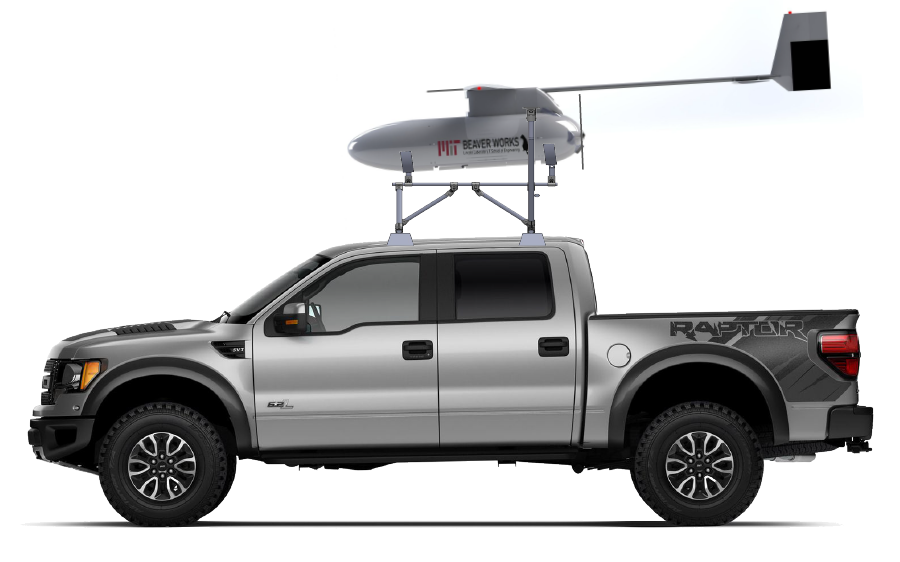
\includegraphics[width = .5\textwidth]{takeoffVehicle.png}
	\caption{The aircraft is mounted on the back of a launch vehicle, which brings the JHO to takeoff speed.}
	\label{f:takeoffVehicle}
\end{figure}

\begin{figure}[h!]
    \begin{center}
    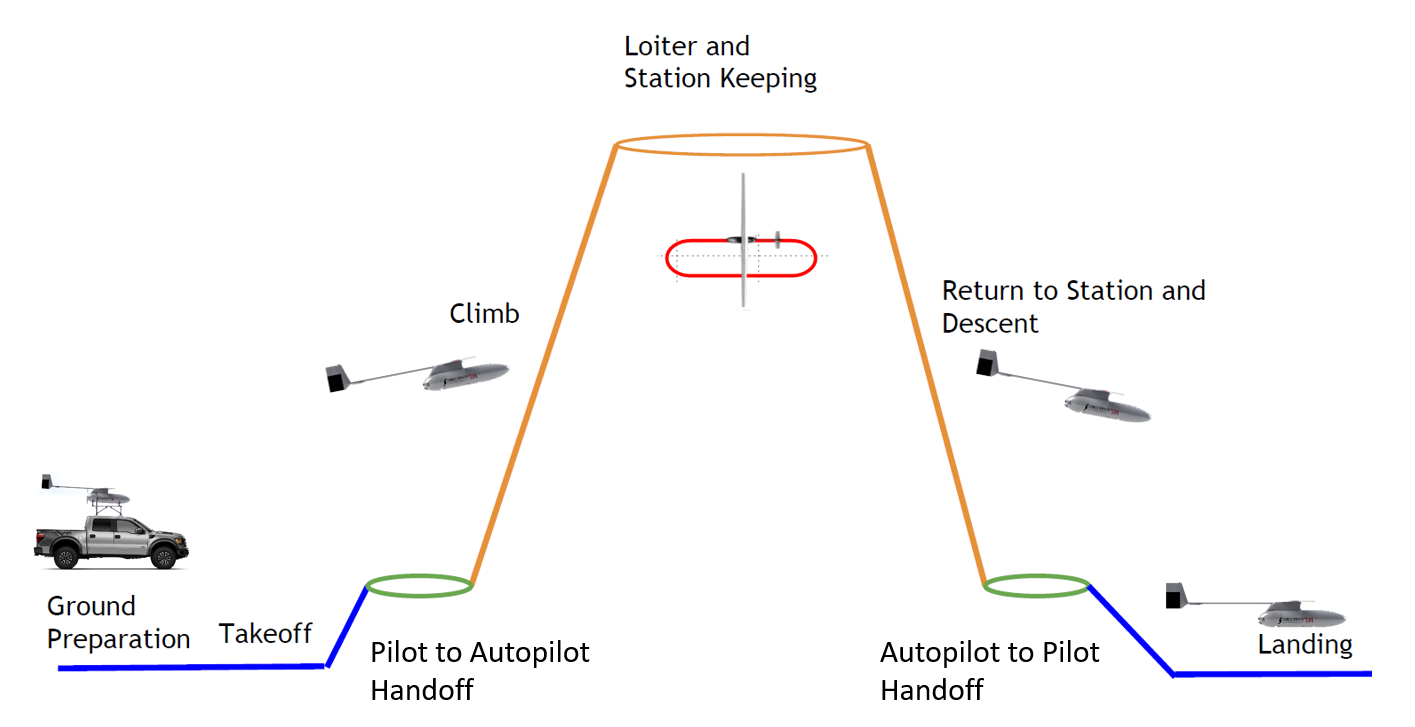
\includegraphics[width = .75\textwidth]{missionProfileLabeled.png}
     \caption{ \textbf{Concept mission profile} }
    \label{f:missionProfile}
    \end{center}
\end{figure}

 Takeoff is performed within visual range of a pilot with direct control of the aircraft through a UHF controller included in the ground station. The vehicle accelerates to the aircraft's takeoff speed, and when it is reached, the pilot performs an aggressive pull-up maneuver at full throttle to allow the aircraft to separate from the vehicle. The aircraft launch requires less than 1050ft of straight road (paved or unpaved) for takeoff, considering the acceleration and braking distance of typical vehicles.

\begin{figure}[h!]
    \begin{center}
    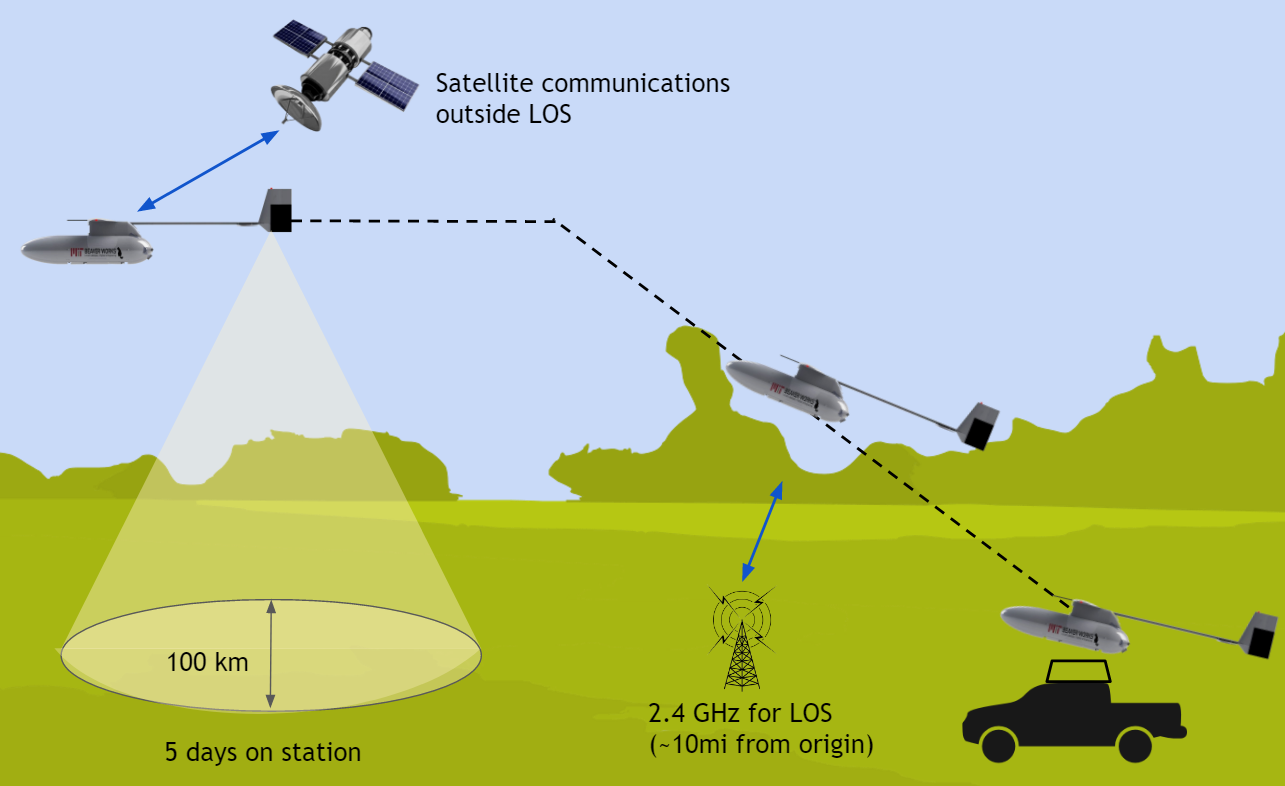
\includegraphics[width = .75\textwidth]{conops}
     \caption{ \textbf{Concept of operations} }
    \label{f:conops}
    \end{center}
\end{figure}

Shortly after takeoff, before the aircraft escapes the UHF communications range of 10 miles from its ground station, the ground-based pilot transfers control authority to the autopilot system. The aircraft climbs autonomously to an altitude of 15,000ft, its loiter altitude. It then cruises up to 200 nmi to its loitering station. 

While on station, the aircraft functions on a trajectory and way point system to autonomously station-keep for the 5-day duration of its mission. The aircraft's payload provides a communication link for land users that are beyond line-of-sight (BLOS).  Communications with the aircraft are maintained through a satellite-based Internet system, which allows operators to receive telemetry about the aircraft's systems. This scheme is shown in Figure~\ref{f:conops}.

At the end of its mission, the vehicle autonomously cruises back to its landing location, and is landed visually by a ground-based pilot using commands through UHF radio. The aircraft landing distance is less than 200ft.

After landing, appropriate maintenance is conducted. The aircraft is able to launch within 6 hours if more communication coverage is required. It is also be possible to coordinate the flight of multiple of aircraft to provide more persistent coverage, or cover adjacent sectors. If the aircraft's mission has concluded, all of the components of the aircraft system are packed, and shipped back to its storage location to await its next mission. 

\section{Requirements}

This section details the requirements of the aircraft fulfilling the concept of operations described in Section~\ref{Concept of Operations}.

\begin{itemize}
    \item \textbf{Endurance: } The minimum endurance is specified at 5 days, for persistent communications coverage. 
    \item \textbf{Availability: } The minimum required availability is 95\%. Availability is defined as the capability of the vehicle to operate in a variety of wind conditions. In addition, the aircraft must be able to fly at any location between $\pm$ 60$^{\circ}$ latitude.
    \item \textbf{Communications coverage area: } The requirement for the payload's communication coverage area is 100 km in diameter, with a 5$^{\circ}$ ground terminal elevation angle. 
    \item \textbf{Range to station: } The aircraft must have the capability to be launched and recovered from a location at least 200 nmi from the station keeping location.
    \item \textbf{Payload: } The aircraft is required to carry a 10lb, 100W payload, and have at least 1 ft$^3$ of payload volume. With future missions in mind, the ability to accommodate various payload sizes, power loads, and modularity are all beneficial, and is a secondary objective.
\end{itemize}

\section{Requirements Analysis}

\subsection{Endurance}

The chosen endurance requirement primarily drives the design of the aircraft. The minimum requirement for endurance is 6 days (144 hours), whereas the current endurance record for a gas-powered UAV belongs to the Aurora Orion, which flew for 80 hours in 2014~\cite{FAIrecords}. As such, the proposed aircraft will be operating at the upper limits of current gas-piston aircraft technology. 

An analysis on the feasibility of solar power to satisfy the above requirements was conducted in the early stages of this aircraft's development. It was concluded that a solar aircraft cannot feasibly achieve the threshold requirements for availability and latitude with currently-available technology, with the worst-case operational scenario being flying in high-wind conditions in the winter solstice. In contrast,a gas-powered aircraft would not be subject to the limitations of the time of year and latitude. Thus, the aircraft proposed here is powered by a piston engine.

For all aircraft, endurance is maximized by minimizing power consumption at the cruise altitude, which requires flying at low airspeeds. To station-keep however, the aircraft has to fly at an airspeed no less than the windspeed at a given altitude. As such, it is beneficial to fly at an altitude with lower winds, which will require less thrust power and lower fuel consumption.

\subsection{Availability and Station Keeping}

   The coverage diameter requirement determines the aircraft's minimum loitering altitude; because the payload uses LOS communication, the loiter altitude is the primary determinant of ground coverage area. Taking into account the curvature of Earth, the minimum 100 km footprint requires flight at 15,100 ft (4.6 km) above ground level. 

    Different altitudes require different propulsive capabilities due to changes in air density and mean winds. As shown in Figure~\ref{f:wind_profiles}, the 95th percentile wind at 15,000 ft is 30 m/s. The wind speed increases linearly for the lower 35,000ft of altitude. For piston engines, it is estimated that an aircraft can operate at up to 22,000ft with a normally-aspirated engine, while higher altitudes require a turbocharger or supercharger to increase the density of the air going into the engine. While these are not necessarily prohibitive, they add cost, weight, and design risk. Therefore, an operating altitude of 15,000 ft was chosen, to satisfy the station keeping and availability requirements with lowest risk and aircraft mass. 
    
\begin{figure}[h!]
\begin{center}
\begin{subfigure}{0.45\textwidth}
    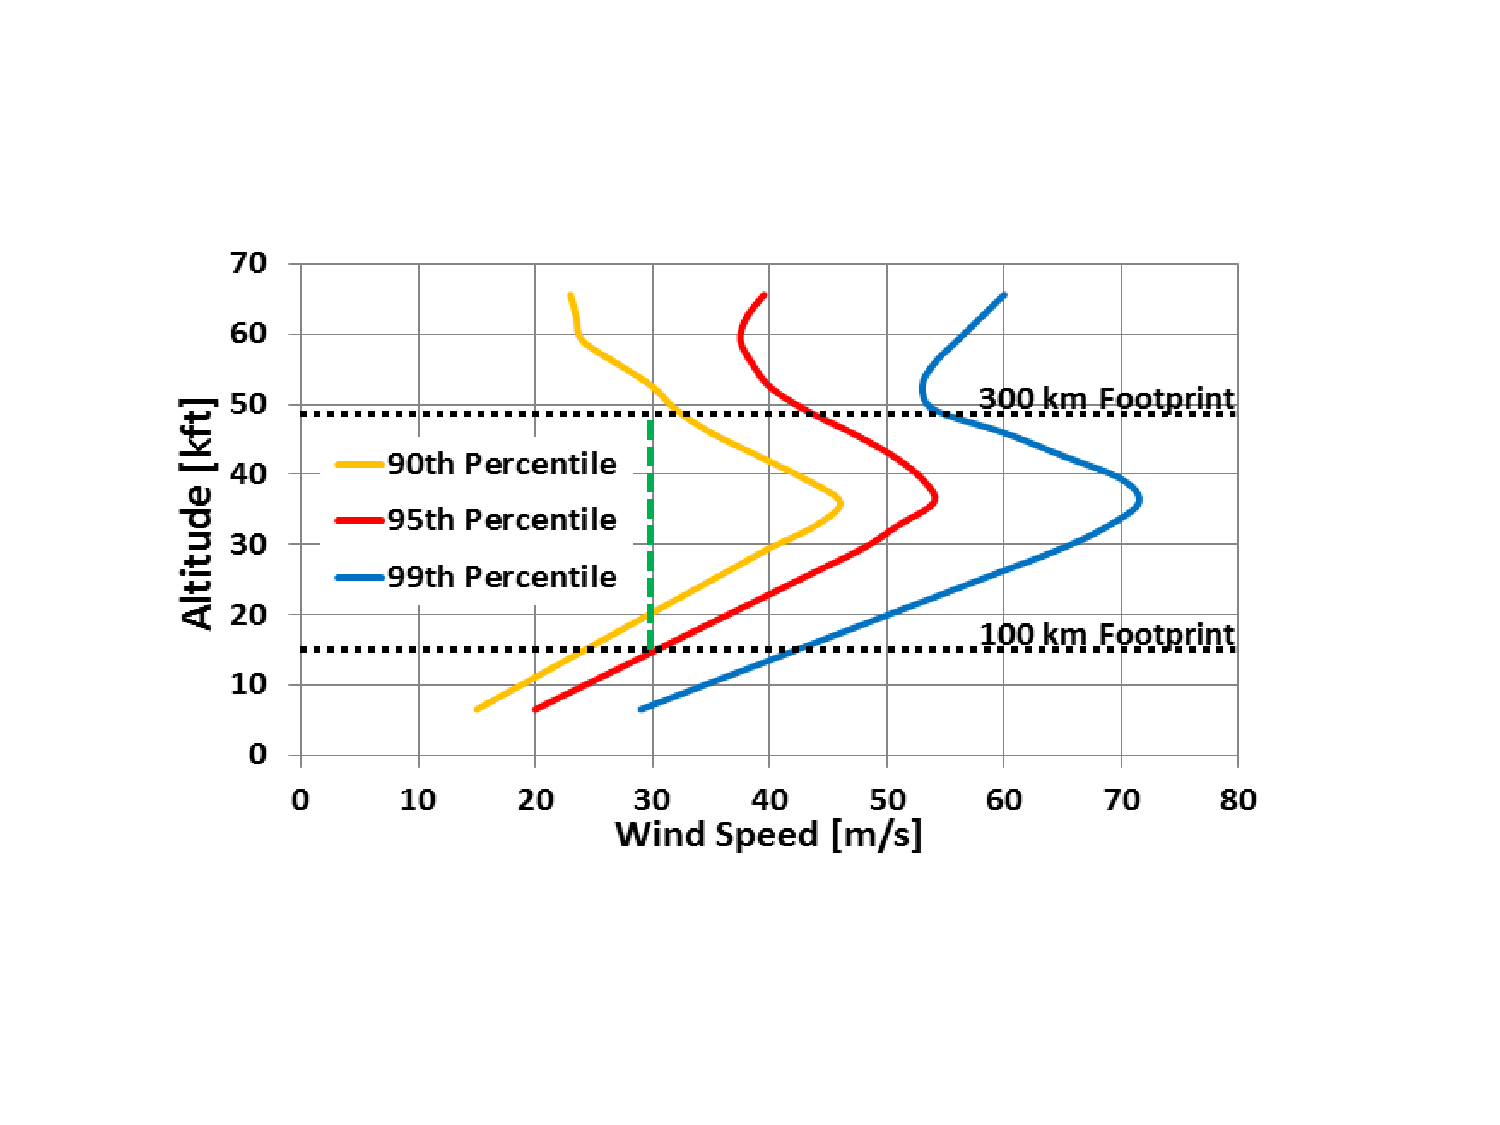
\includegraphics[width = .9\textwidth]{wind_profiles}
    \caption{ \textbf{The global 90th, 95th and 99th percentile winds as functions of altitude.} }
    \label{f:wind_profiles}
\end{subfigure}
\begin{subfigure}{0.45\textwidth}
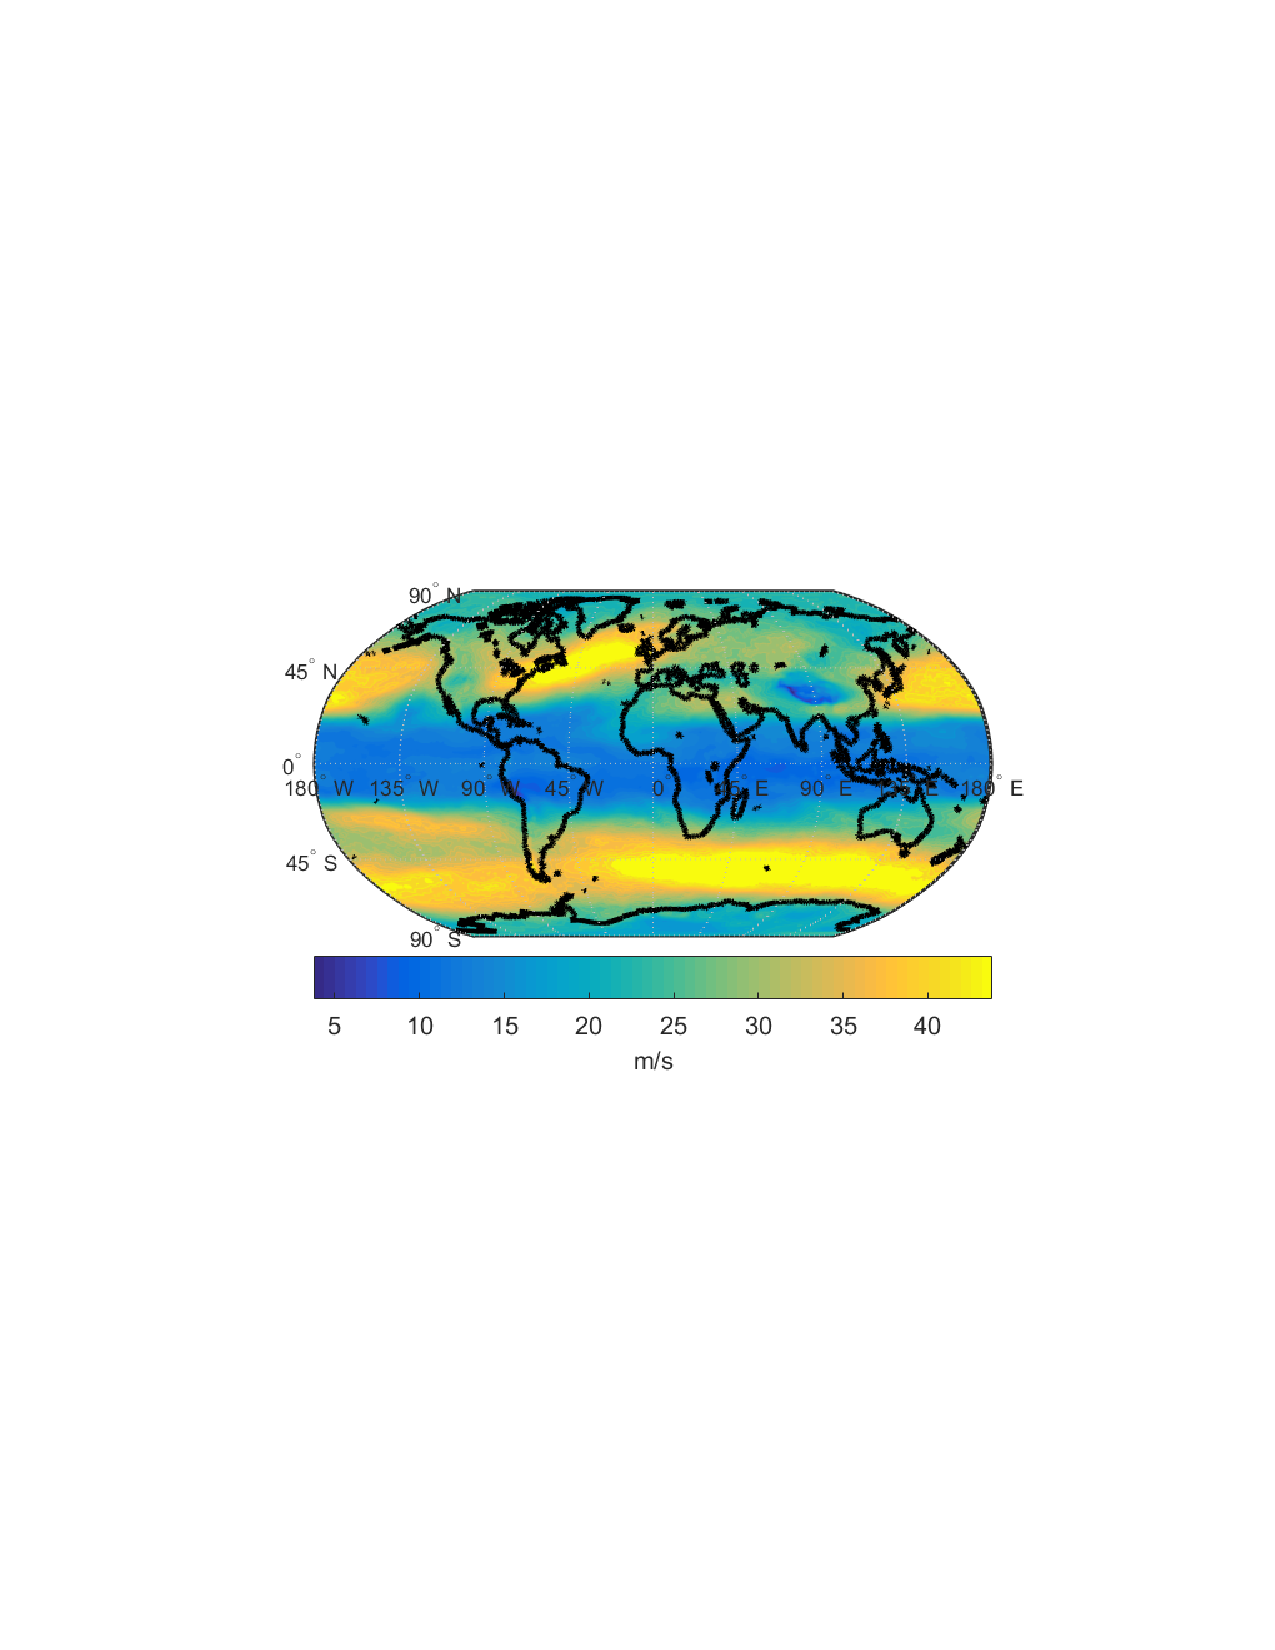
\includegraphics[width = .8\textwidth]{wind_map}
    \caption{ \textbf{Map of 95th percentile winds at 15,000 ft in 2015.} }
    \label{f:wind_map}
\end{subfigure}
\end{center}
\caption{Winds determine aircraft availability. Source: European Center for Medium-Range Weather Forecasts}
\label{f:winds&availability}
\end{figure}

\subsection{Latitude, Range to Station and Implicit Requirements}

The loiter velocity of the aircraft is coupled to winds aloft. As a result, it is critical to to examine local trends in wind speed with altitude, as well as the global trends. A map of the 95th percentile winds at 15,000 ft is shown in Figure~\ref{f:wind_map}. It can be noted that the windiest locations are over the oceans between the 30th and 60th parallels. Since the mean wind speed over land (and populated areas) is lower than that over the oceans, we expect that an aircraft designed for 90\% availability globally (25 m/s loiter airspeed) will achieve the 95\% availability requirement in its design mission. 

In addition, aircraft modularity was implicitly required in order to allow for easy shipping of the aircraft to its launch location. And while aircraft cost is not a specified requirement for this project, the aircraft must be cost effective. Studies have shown that aircraft cost is proportional to aircraft weight \cite{costeco}. As such, for this aircraft, minimizing maximum takeoff weight (MTOW) will result in lower operational costs. 

\section{Vehicle Sizing and Optimization}
\label{Vehicle Sizing and Optimization}

There were important multidisciplinary trade-offs that needed to be understood in order to correctly size the proposed aircraft. To explore these trade-offs, an optimization tool called GPkit was used. GPkit is a convex optimization framework that leverages Geometric Programming (GP)~\cite{GPkit}.

GP is a special form of optimization in which the constraints of the aircraft system are expressed in monomial and posynomial forms. The general form of a GP problem is shown in Equation~\ref{e:gpform},

\begin{align} 
\label{e:gpform}
\text{minimize } f_0(\mathbf{x}) & \nonumber \\
\text{subject to  } f_i(\mathbf{x}) &\leq 1, i=1,...,m \\
g_i (\mathbf{x}) &= 1, i = 1,...,p \nonumber
\end{align}
 
 where the functions $f_i$ must be \emph{posynomial} functions and the functions $g_i$ must be \emph{monomial} functions. \emph{Monomials} and \emph{posynomials} have the forms
 
\begin{align}
\label{e:mon}  g(\mathbf{x}) &= c x_1^{a_1} x_2^{a_2} \dotsm x_n^{a_n} , \\  \label{e:pos}  f(\mathbf{x}) &= \displaystyle\sum_{k=1}^K c_k x_1^{a_{1_k}} x_2^{a_{2_k}}
\dotsm x_n^{a_{n_k}}.  
\end{align}

This optimization framework allows for the synergistic design of all subsystems of the aircraft. In the design of the UAV, each subsystem (aerodynamics, structures, propulsion, avionics, operations) contributed different models and governing equations specific to their discipline. These models were converted into the GP-compatible forms aforementioned, and were integrated systematically into the optimization model. 

\subsection{Configuration Overview}

The assumed configuration for the GP models is a fixed-wing aircraft in a pusher configuration with a conventional tail. The aircraft structure consists primarily of composites. A single-cylinder internal combustion engine drives the propeller and the alternator, generating thrust, and electrical power for the avionics and payload. The vehicle has a pylon-mounted wing, with an integrated engine intake for both aspiration and cooling. The vehicle can be remotely piloted, or operated autonomously via autopilot. Figure~\ref{f:features} overviews the notable design features of the aircraft.

\begin{figure}[h!]
    \begin{center}
    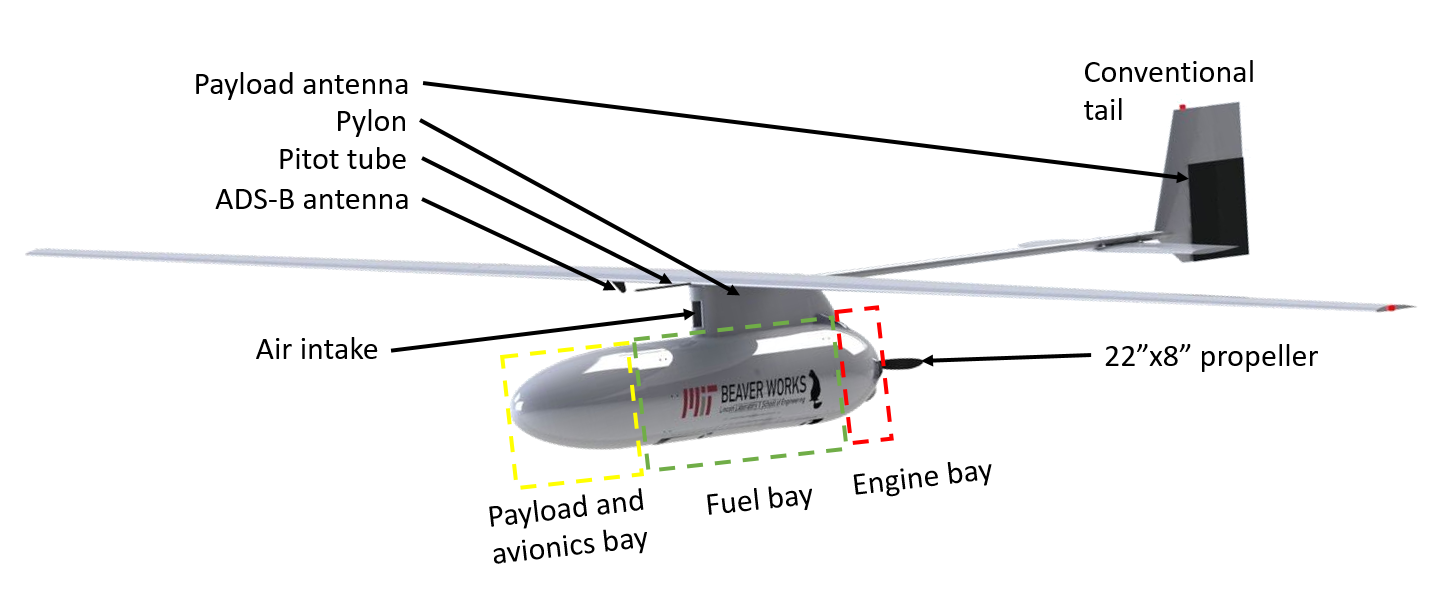
\includegraphics[width = .75\textwidth]{features}
     \caption{ \textbf{Notable design features of the aircraft} }
    \label{f:features}
    \end{center}
\end{figure}

A 1.43 cubic-foot payload bay is placed in the nose of the vehicle, presenting an unobstructed location for payload and sensor mounting. We chose a pusher configuration to eliminate the effects of scrubbing drag.

Traditional landing gear configurations were foregone for a shock-absorbing rear landing wheel and a forward landing skid because analysis showed that the weight and drag added by a tricycle landing gear would have increased the fuel required to achieve the 6 day mission endurance by up to 17\%. This decision required the design of a non-traditional, effective landing and takeoff system. 

For takeoff, we propose a vehicle-assisted takeoff scheme, detailed in Section~\ref{Concept of Operations}. For landing, the front landing skid and the rear wheel have been designed to dissipate the vertical kinetic energy of the impact by compressing shock-absorbing rubber stoppers through a stroke distance. Furthermore, the wing tips of the aircraft are reinforced to be able to withstand a wingtip strike.

There are implicit requirements for the aircraft from an operations perspective. The potential for the vehicle to be deployed around the world necessitates modularity and ease of transport. There was no straightforward method to implement modularity constraints within the optimization framework. But further analysis on the modularity of the design was done post-optimization, and is presented in Figure \ref{f:modularity} in Section~\ref{Appendix}. This allows the packaged aircraft, its ground station and launch systems to be transported around the world within 24 hours, ready to be deployed in a moment's notice. 

\subsection{Modeling Assumptions}
The following are the assumptions used in the design optimization of the proposed aircraft, along with a brief justification as to why each assumption was made. 

 \subsubsection{Mission Profile:} The mission profile (also outlined in Section~\ref{Concept of Operations}) starts with a climb to 15,000ft. During the climb phase, the engine is required to supply the necessary power to provide a constant climb rate of at least 100 ft/min. The aircraft then cruises 200 nmi to the loitering station. Upon arriving there, it starts loitering, providing a communication coverage footprint of 100 km for a minimum of 6 days. Then it cruises back to its point of takeoff. The plane was modeled to be in steady flight during all phases of the mission. We assumed that the propeller efficiency was constant during each phase, with a conservative average efficiency of 68\% in cruise. 
 
 \subsubsection{Engine Weight and Power: }  The engine size and available engine power were based off a power-law regression fit to a dataset of two and four stroke, gas piston engines.  Figure~\ref{f:powervsweight} shows the weight and power distribution of the data used in the regression. 
 
\begin{figure}[h!]
    \begin{center}
    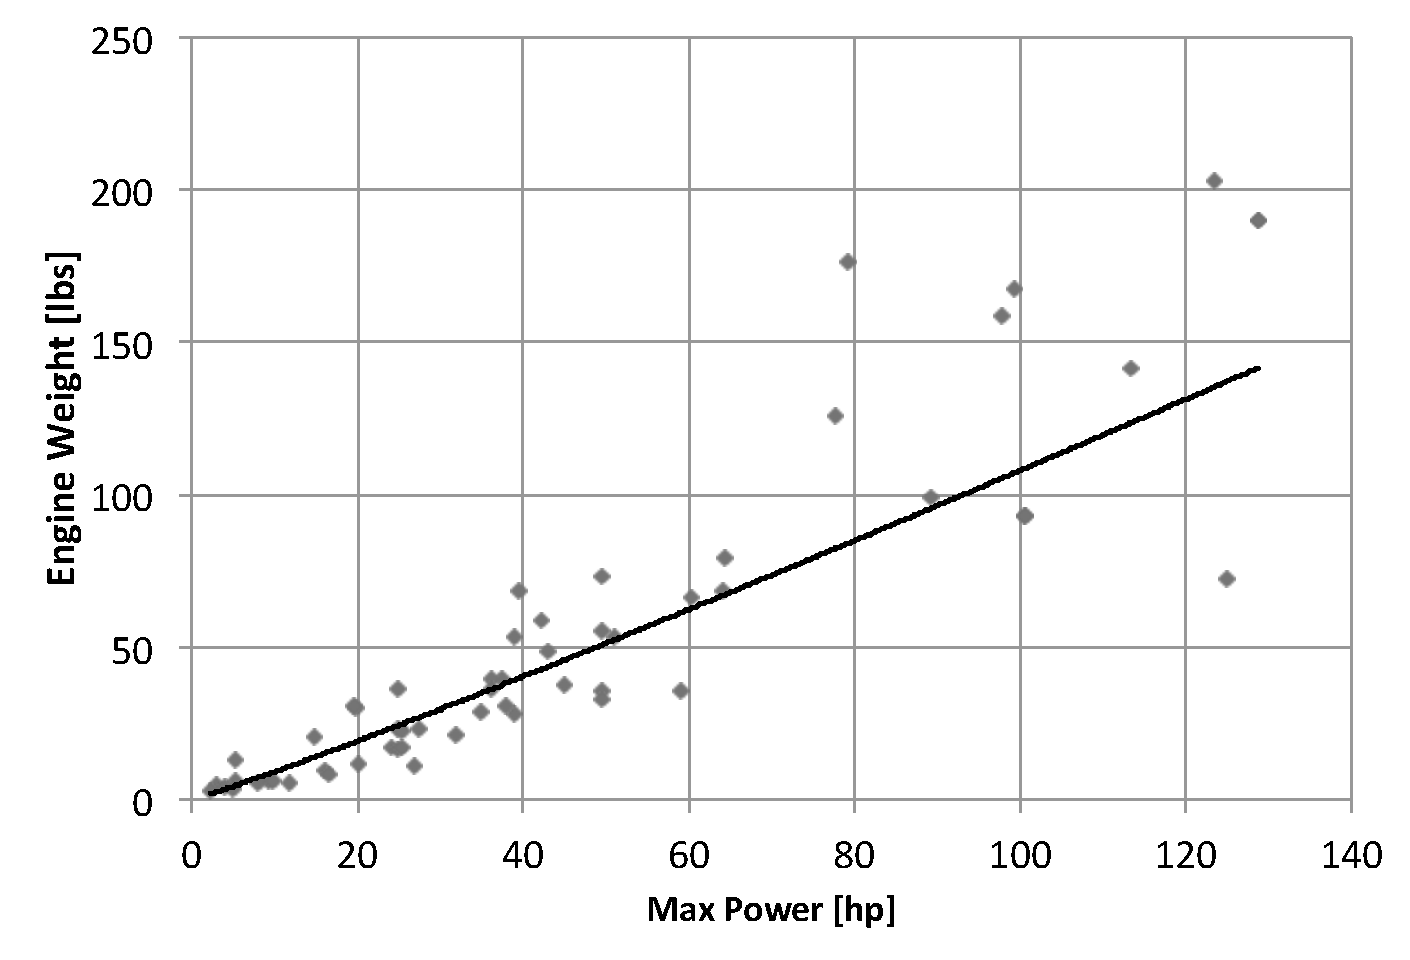
\includegraphics[width = .65\textwidth]{powervsweight}
    \caption{ \textbf{Weight versus power curve for small reciprocating engines.\cite{smallengines} The trendline is a monomial approximation of the available engine data.} }
    \label{f:powervsweight}
    \end{center}
\end{figure}

Furthermore we assumed that the engine performance could be approximated by the curves shown in Figure~\ref{f:engineperf}. We used data provided by RCV Engines Ltd., a small reciprocating UAV engine company, to validate the models. Figure~\ref{f:engineperf} shows the the models for the power lapse rate and efficiency of naturally-aspirated piston engines. 

\begin{figure}[h!]
    \begin{center}
         \begin{subfigure}{0.45\textwidth}
             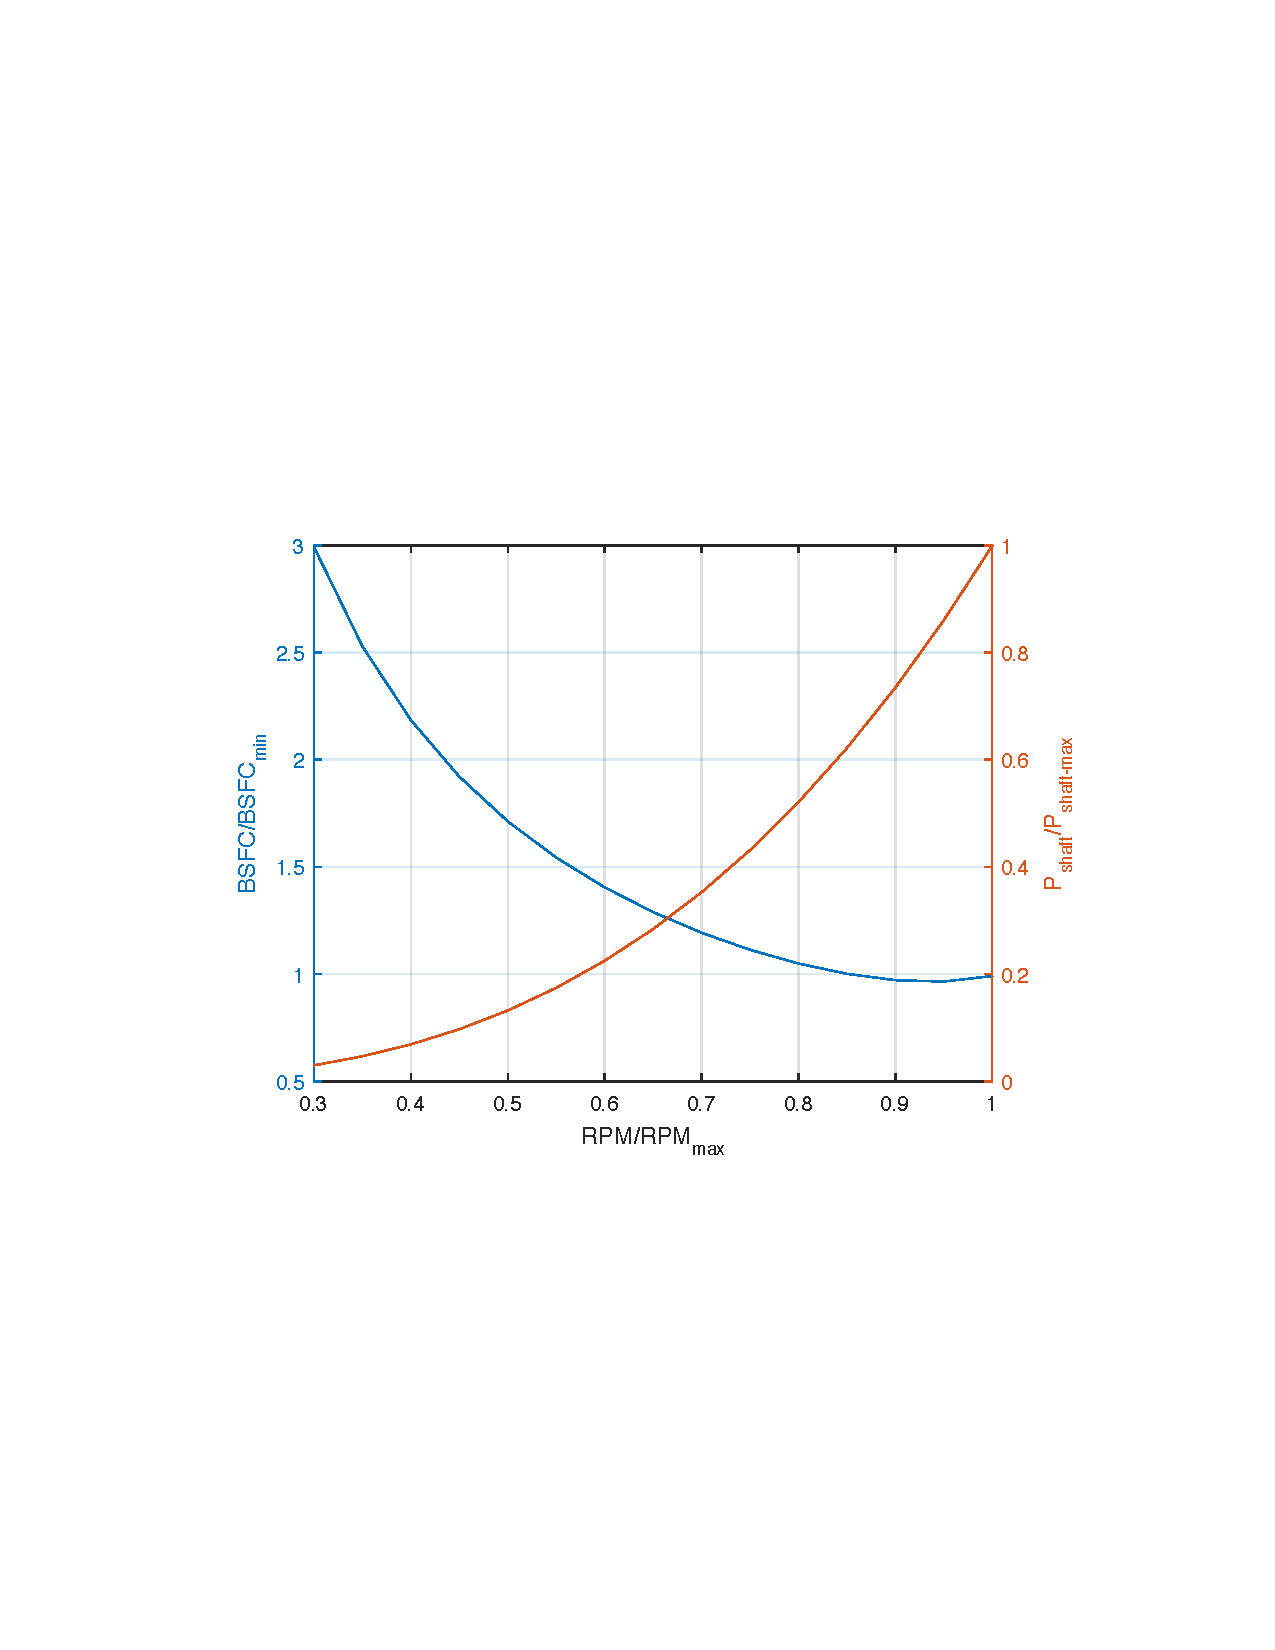
\includegraphics{BSFC_P_shaftvsRPM}
             \caption{ \textbf{BSFC and shaft power relations to RPM} }
         \end{subfigure}
         \begin{subfigure}{0.45\textwidth}
            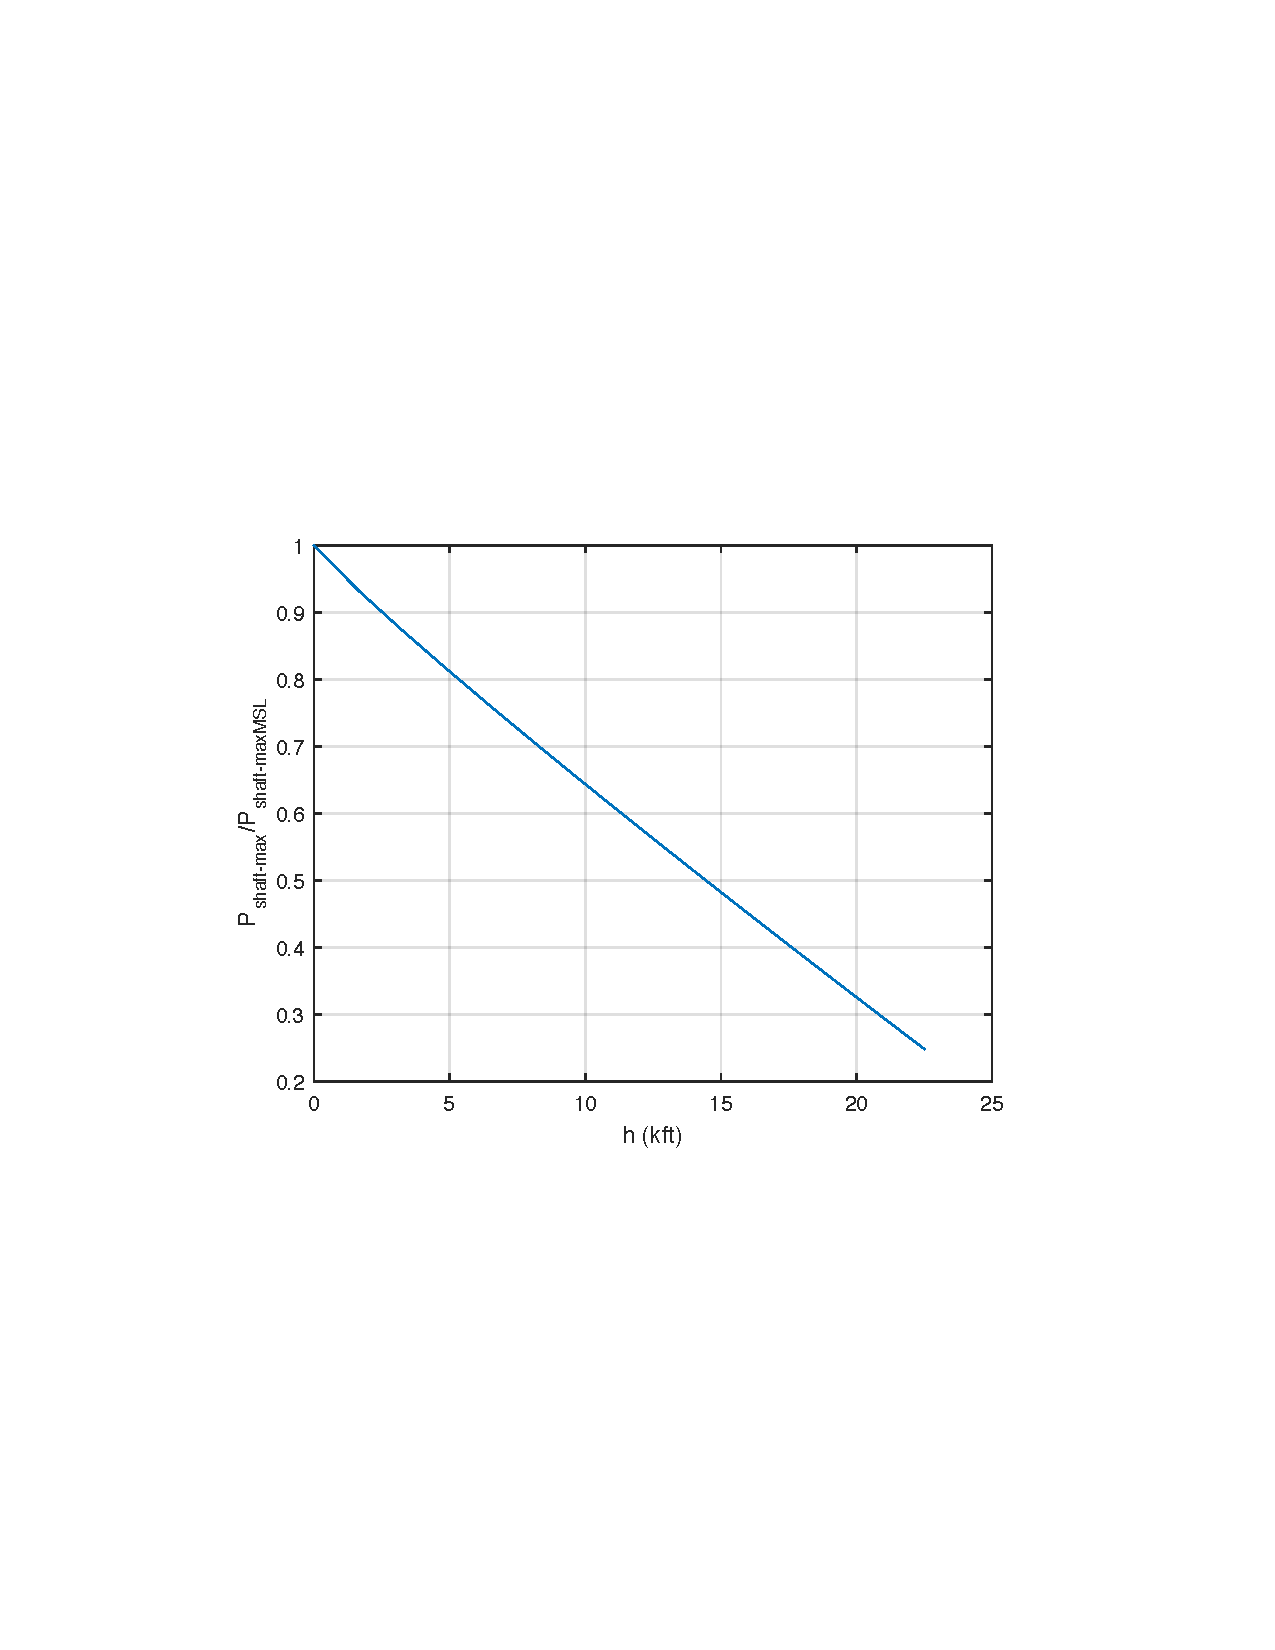
\includegraphics{P_shaftvsh_station}
             \caption{ \textbf{Engine power lapse rate with altitude} }
         \end{subfigure}
         \caption{ \textbf{Assumed engine performance of small piston engines} }
    \label{f:engineperf}
    \end{center}
\end{figure}

\subsubsection{Aerodynamics}

The wing is assumed to be manufactured out of 3 equal-span wing sections. It is a constant taper wing with a taper ratio of 0.5, which provides a good compromise between structural design and span efficiency. There is no dihedral built into the design; it is estimated that the tip deflection of the aircraft under loading, combined with its high-wing configuration, provide enough roll stability to make extra dihedral unnecessary.

The empennage of the aircraft is a conventional tail configuration. Configuration studies were conducted to see the relative performance of three different designs, namely an inverted-V tail, a pi tail, and dual dart tails. However, the potential interference of the payload patch antenna with the aircraft's carbon fiber structure and rotating metal parts necessitated the placement of the antenna on the vertical tail, as shown in Figure~\ref{f:features}. This posed constraints on the minimal dimensions of the vertical tail, which resulted in the conventional tail design outperforming the other concepts. The horizontal tail is sized for 100\% CL margin for maximum forward CG of the aircraft (maximum payload of 15 lbs). The vertical tail is sized using a tail volume coefficient. The vertical tail has a small downward offset to reduce the interference of the antenna with the fuselage, without causing potential tail-strikes. 
     
The set of control surfaces consists of an aileron on each side of the wing, two elevators on the horizontal tail, and a rudder on the vertical tail. The control surfaces are sized for sufficient control authority at $V_{stall}$, and the associated actuators are sized for maneuvers at the never-exceed speed of 40 m/s indicated.  This analysis for control surface loading was conducted using XFOIL\cite{XFOIL}. 

We assume that drag is a sum of the fuselage drag, the wing profile drag, the engine cooling drag, and the induced drag of the aircraft.  The induced drag is calculated from the lift required by the aircraft, assuming an Oswald efficiency of 95\%.

\begin{itemize}
    \item \textbf{Fuselage Drag:} 
    The fuselage was modeled in MTFLOW, an axisymmetric version of XFOIL, which gave a values for $C_{D_{fuselage}}$ of 0.0028 and 0.0032 for a laminar nose and a turbulent nose (tripped at the leading edge to ensure full turbulence) in the loiter condition, respectively. A Blasius turbulent flat plate model, with an associated form factor correction (fineness ratio of 6.5), is implemented in the GPkit model to extrapolate the drag coefficient to other flight conditions. 
    
    \item \textbf{Wing and Tail Profile Drag:}
    The wing profile drag equation was based off of the drag polars of the JH01, JH02, and JH03 airfoils, created in XFOIL\cite{XFOIL} (a two-dimensional computational fluid dynamics program), and is a function of the lift coefficient and Reynolds number. Figure~\ref{f:4_JH01_Polars2} shows the airfoil drag polar used to calculate the wing profile drag. These airfoils are variants of the remote controlled (RC) glider airfoil SD7032 suitable for higher Reynolds number operation and a larger airfoil thickness ratio. The pressure distributions of the airfoils at maximum and minimum lift coefficients are shown in Figure~\ref{f:JHpressure}. Similarly, the drag polar for the symmetric NACA0008 airfoil was used to calculate the profile drag of the tail surfaces. 
    
    \item \textbf{Cooling Drag: }
    The cooling drag is estimated by a first principles model that satisfies engine cooling requirements. 
    
    \item \textbf{Drag Margin:} 
    To account for other potential sources of drag (interference drag, manufacturing imperfections etc.) there is a 0.002 margin added to the $C_{D0}$ of the aircraft. 
    
    \item \textbf{Total Vehicle Drag:}
    The total vehicle drag is the sum of the individual sources mentioned above:
    
    \begin{equation}
            \label{e:totaldrag}
            C_D = C_{D_{profile}} + \frac{C_L^2}{\pi e AR} + C_{D_{fuselage}} + C_{D_{cooling}} + C_{D_{0}} 
    \end{equation}
\end{itemize}

    \begin{figure}[h!]
    \begin{center}
    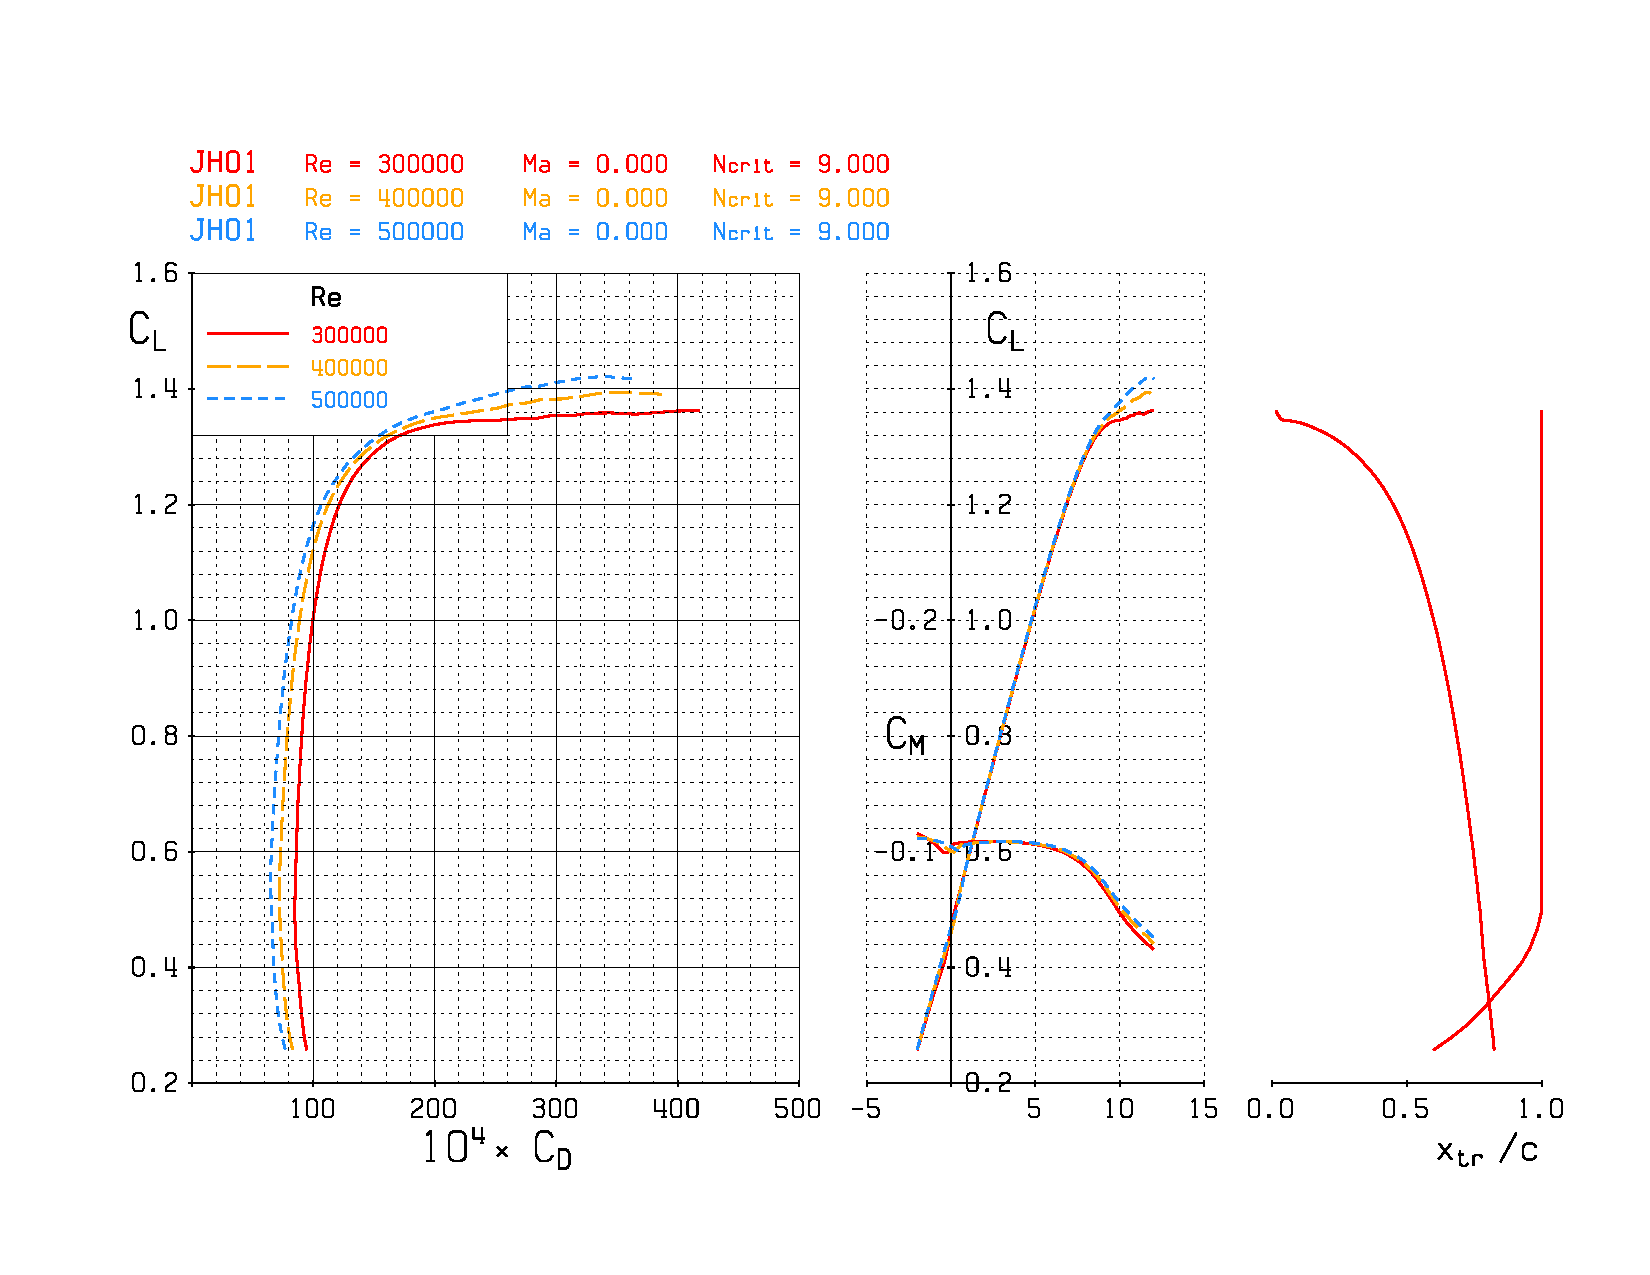
\includegraphics[width = .75\textwidth]{4_JH01_Polars}
     \caption{ \textbf{Drag polars for the JH01 airfoil at $Re = 3e5-5e5$} }
    \label{f:4_JH01_Polars2}
    \end{center}
    \end{figure}
    
    \begin{figure}[h!]
    \begin{center}
         \begin{subfigure}{0.49\textwidth}
             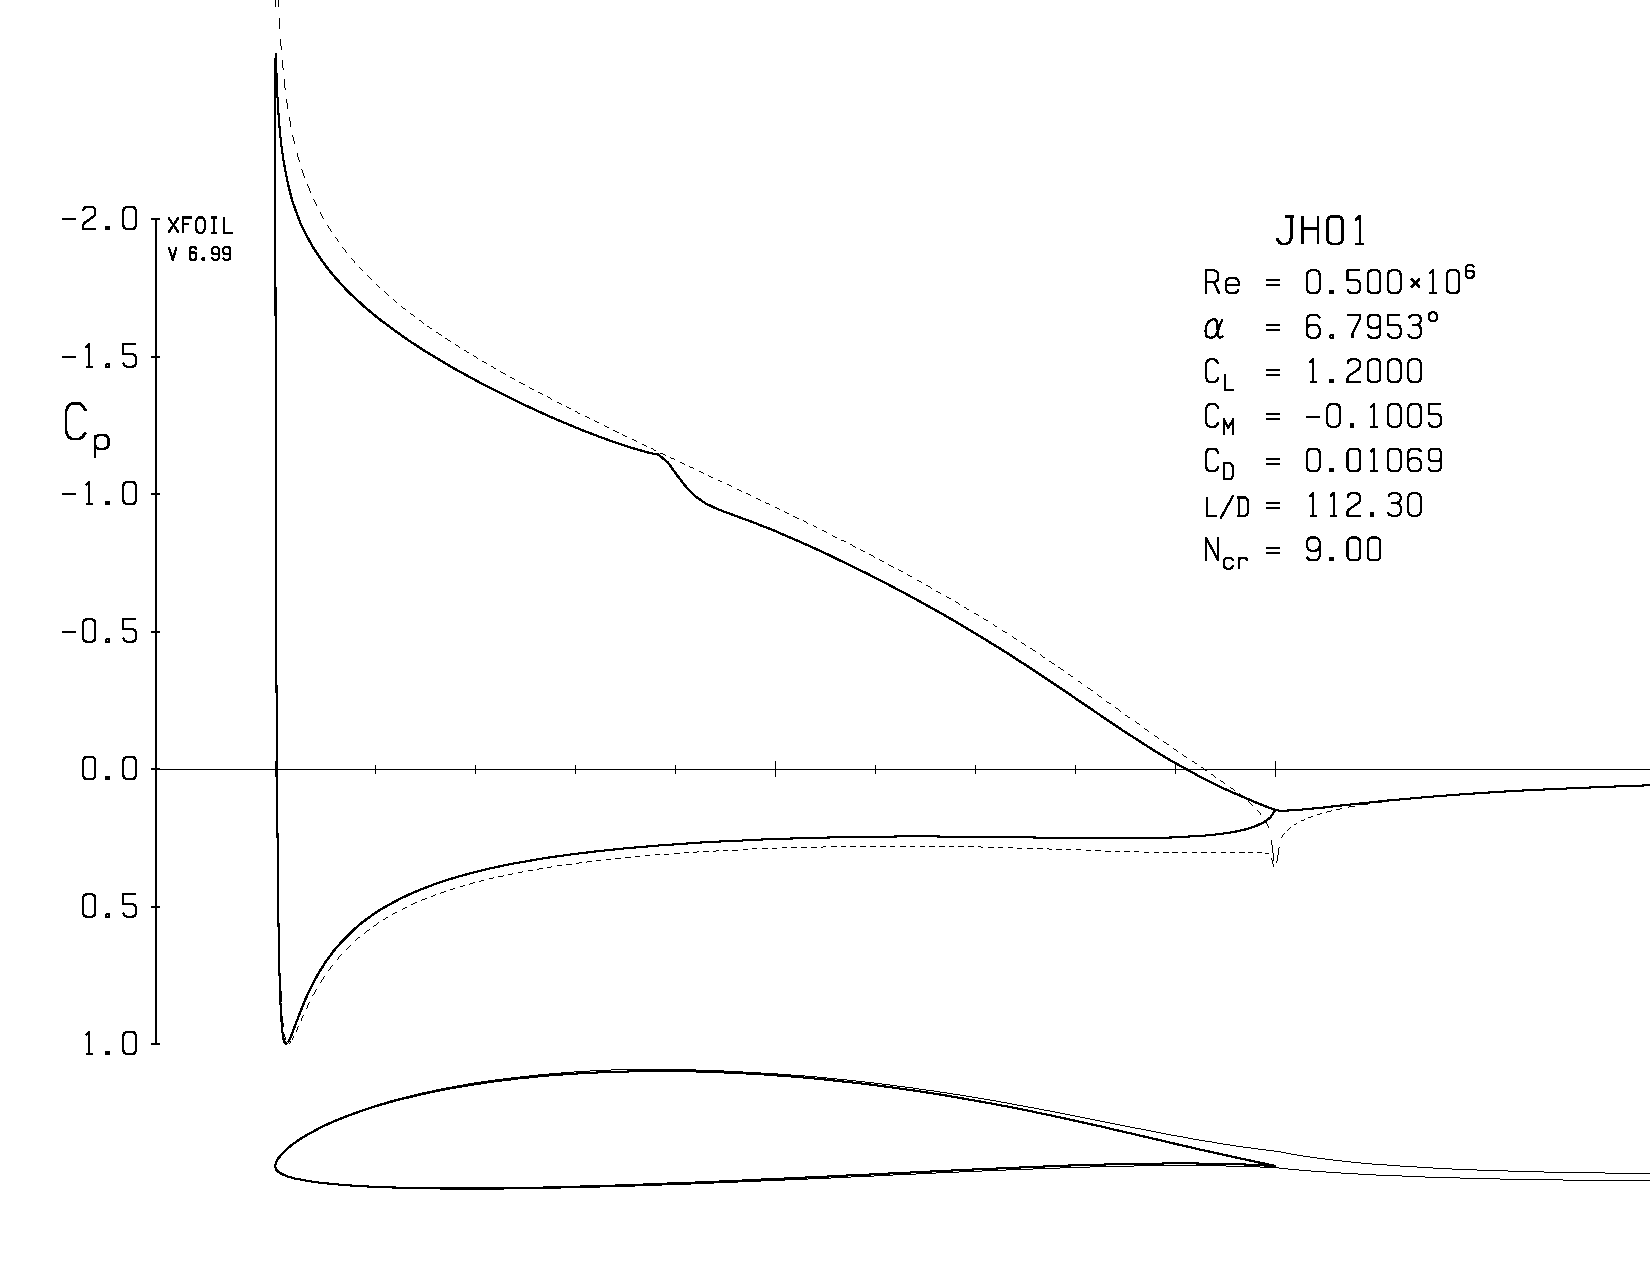
\includegraphics{5_JH01_maxCl}
             \caption{ \textbf{Max Operating CL }}
         \end{subfigure}
         \begin{subfigure}{0.49\textwidth}
             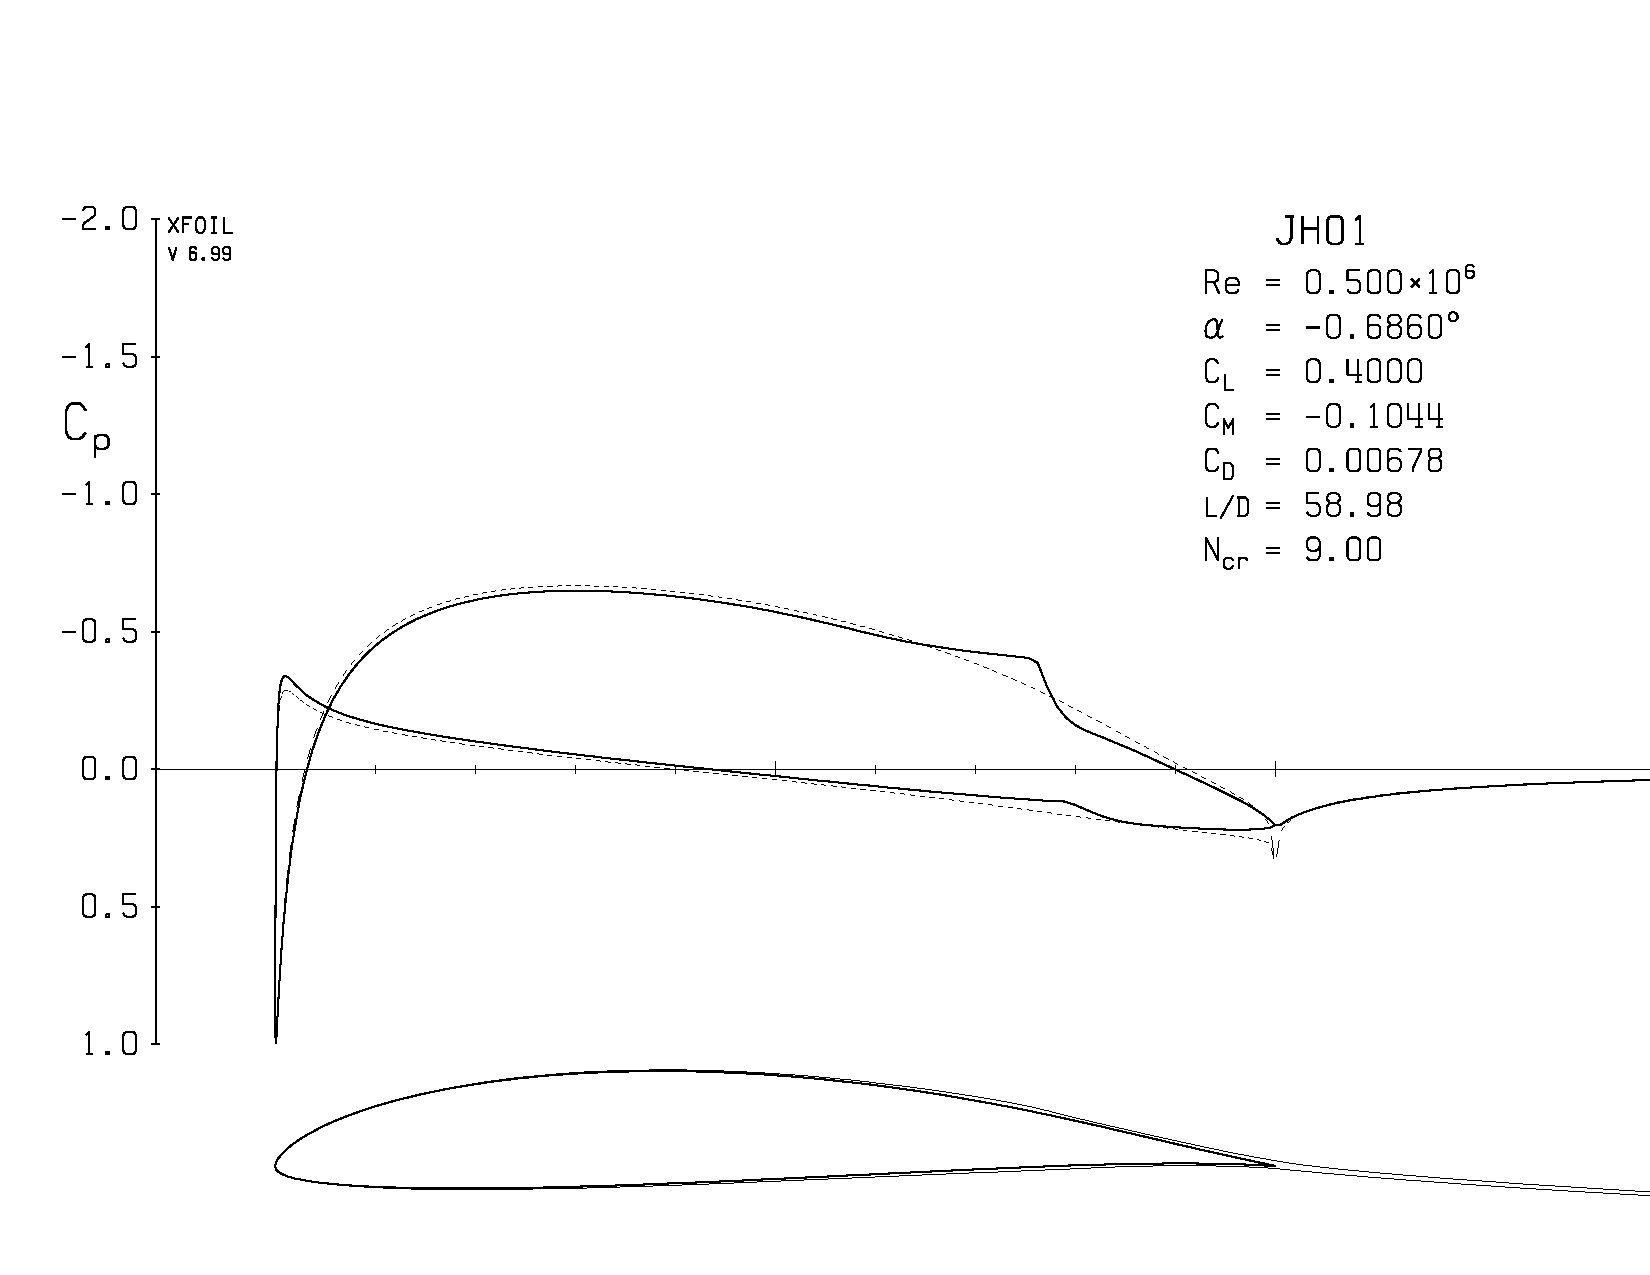
\includegraphics{6_JH01_minCL}
             \caption{ \textbf{Min Operating CL} }
         \end{subfigure}
         \caption{ \textbf{Pressure Distributions for the JH01 airfoil at maximum and minimum operating $c_l$} }
    \label{f:JHpressure}
    \end{center}
    \end{figure}
    
\subsubsection{Avionics Weight and Volume:} We assume that the avionics weight is 8 lbs, occupies a volume of 0.125 cubic feet, and draws 40W of mean electrical power. We base the estimate on the avionics and batteries needed for actuators, ground communication, satellite communication, alternators, and flight control computers.

\subsubsection{Structures} 

The structural design of this aircraft is driven by the need for a lightweight structure that is modular and allows for payload flexibility. The aircraft is designed with composite materials (Kevlar, carbon fiber, and fiberglass).

\begin{itemize}
    \item \textbf{Wing: } The wing of this aircraft has a solid foam core construction, with carbon front and rear spars, and carbon skin. The spars are sized such that the front spar is capable of withstanding all the bending loads resulting from a 5 g pull-up maneuver with a maximum wing tip deflection that is less than 20\% of the wingspan. The spar height and cap sizing are performed such that the beam would also be able to sustain the root moment from the same load factor without failure. Since the main structural bending element of the wings is the carbon fiber spar, the aerodynamic skin is made with minimum gauge carbon. 
    
    \item \textbf{Tail: } The tail is constructed from a solid foam core with a Kevlar skin, similarly to the wing. Since the tail sections have a smaller aspect ratio and significantly lower loading, no other structural elements are required. The tail booms are sized by constraining the maximum deflection of the tip of the boom during maneuvers at the never-exceed speed of 40 m/s at MSL. 
    
    \item \textbf{Fuselage: } The fuselage is assumed to hold the payload, avionics, batteries, fuel tanks, and the propulsion system. The engineering drawing of the fuselage is shown in Figure~\ref{f:fuselage}. The important features of the fuselage are detailed below: 

    \begin{figure}[h!]
        \begin{center}
        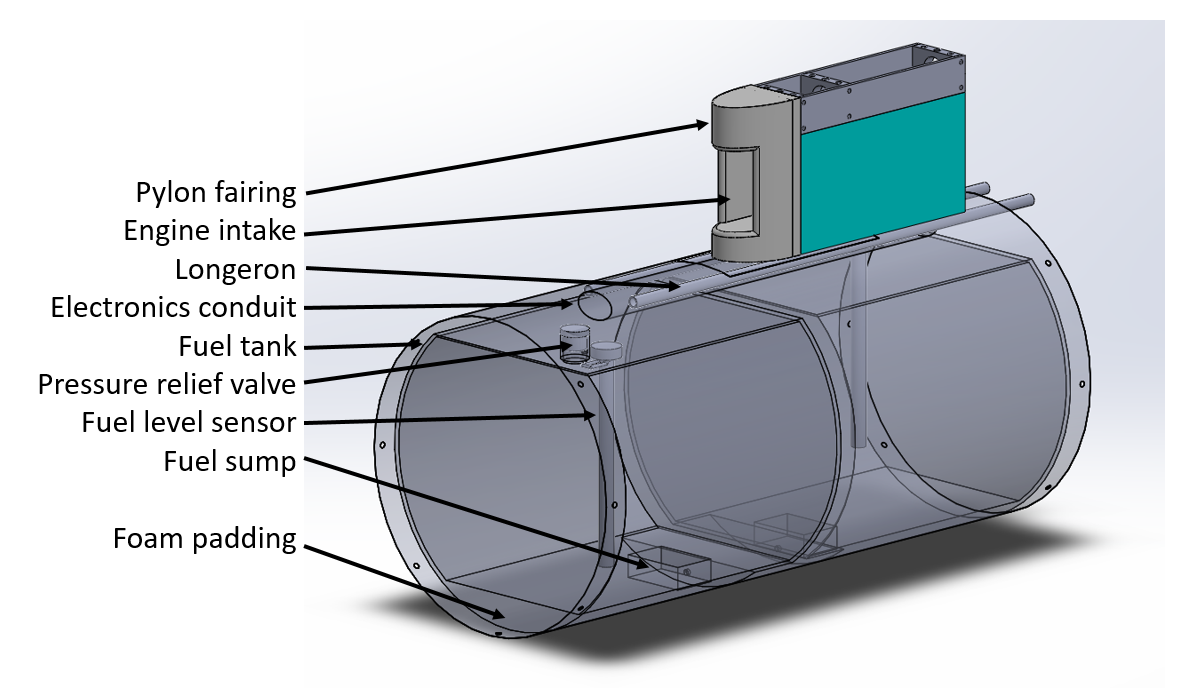
\includegraphics[width = .75\textwidth]{fuselageLabeled}
         \caption{ \textbf{Fuselage layout. The carbon fiber skin has been made transparent to show internal structure.} }
          \label{f:fuselage}
         \end{center}
    \end{figure}
    
\begin{itemize}
    \item \textbf{Pylon: } 
    The pylon contains the air intake and cooling duct, and transfers the aerodynamic loads from the wing and the tail into the fuselage. These loads are transferred into the structural shell of the fuselage through two longerons and a foam bed near the top of the body. It is also designed to take any torsional loads that may result from a wingtip strike upon landing. A CAD of the proposed design is shown in Figure~\ref{f:pylon}.
    
    \begin{figure}
    	\centering
    	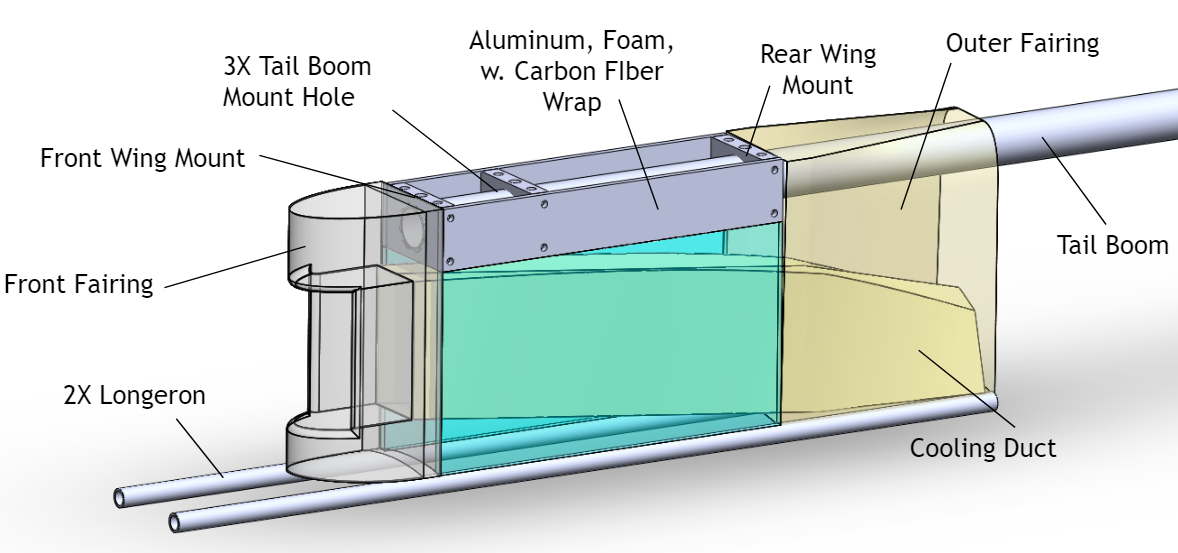
\includegraphics{pylon.PNG}
    	\caption{The pylon provides a structural connection between the wing, fuselage and tail, and houses the cooling duct.}
    	\label{f:pylon}
    \end{figure} 
    
    \item \textbf{Fuel tanks: } 
    The fuel tanks sit below the pylon, so that their CG  is coincident to the aircraft's overall CG. The fuel volume has been separated into two bays to mitigate static stability issues that may result from fuel movement when the aircraft is pitched. 
    
    \item \textbf{Rear landing wheel:} 
    Underneath the rear bulkhead is a wheel which is the first point of contact of the aircraft upon landing, and is designed to absorb the loads experienced during a fully-fueled landing. The wheel structure is made of aluminum, and when it impacts the ground, compresses a rubber stopper that mitigates landing g-loads and dissipates the vertical kinetic energy of the aircraft. A diagram of the setup is shown in Figure~\ref{f:landingGear}.
    
    \begin{figure}
    	\centering
    	\begin{subfigure}{0.45\textwidth}
    		\centering
			 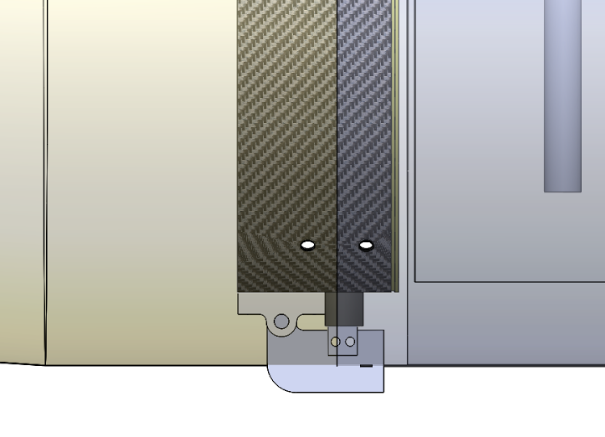
\includegraphics[width = 0.75\textwidth]{frontLandingGear.png}
			 \caption{Front landing gear  is under the front bulkhead}
		\end{subfigure}
		\begin{subfigure}{0.45\textwidth}
		    \centering
		    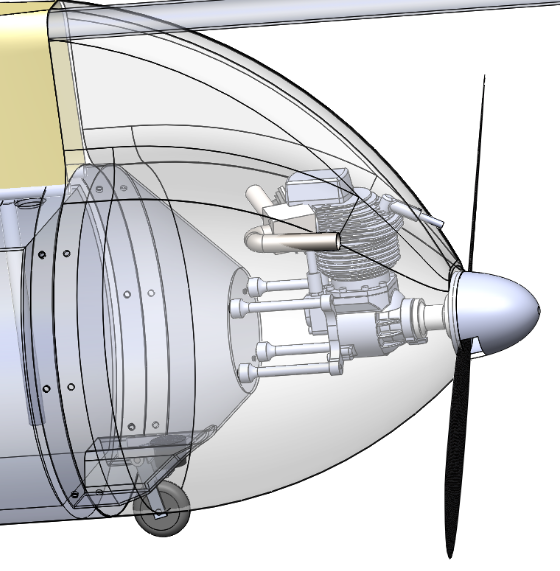
\includegraphics[width = 0.75\textwidth]{rearLandingGear.png}
		    \caption{Rear landing gear is nestled in the rear bulkhead and engine fairing}
		\end{subfigure}
		\caption{Landing gear and engine configuration of the JHO. Rear fairing is transparent to show internals.}
		\label{f:landingGear}
    \end{figure}
    
    \item \textbf{Front landing skid:}
    Underneath the front bulkhead is a blade which functions with the same principle as the rear wheel, absorbing the residual vertical kinetic energy of the aircraft post rear-wheel touchdown. 
    
    \item \textbf{Engine bay: } 
    The engine is mounted on a conical carbon-fiber mount attached to the rear bulkhead, as shown in Figure~\ref{f:landingGear}. The mount has been designed to mitigate engine vibrations, and also to accommodate the routing of the cooling duct into the engine.
    
    \item \textbf{Payload and avionics bay :} 
    The payload and avionics are mounted to the front bulkhead. The front bulkhead has a series of concentric rings of holes which facilitate different payload mounting schemes.
     
    \item \textbf{Aerodynamic fairings: } 
    The aerodynamic fairings around the payload and avionics bay, and the engine, are made of single ply, 0.012" bidirectional carbon fiber. These components are not load-bearing, since the components in the bays are mounted directly onto the bulkheads connecting to the structural fuselage shell. 
\end{itemize}
\end{itemize}

\section{GPkit Optimization}
\label{GPkit}

    From the above assumptions and margins, the sizing problem is defined by a set of constraints that govern the system. To be able to formulate the design as a geometric program, all of the constraints were expressed in monomial and posynomial forms. The objective function was set to maximize the time on station, with all design variables free, including the engine.  Then, by varying MTOW it was observed how the time on station was affected by the size of the aircraft.  Figure~\ref{f:tvsmtow} shows the tradeoff of time on station versus MTOW. 

\begin{figure}[h!]
    \begin{center}
    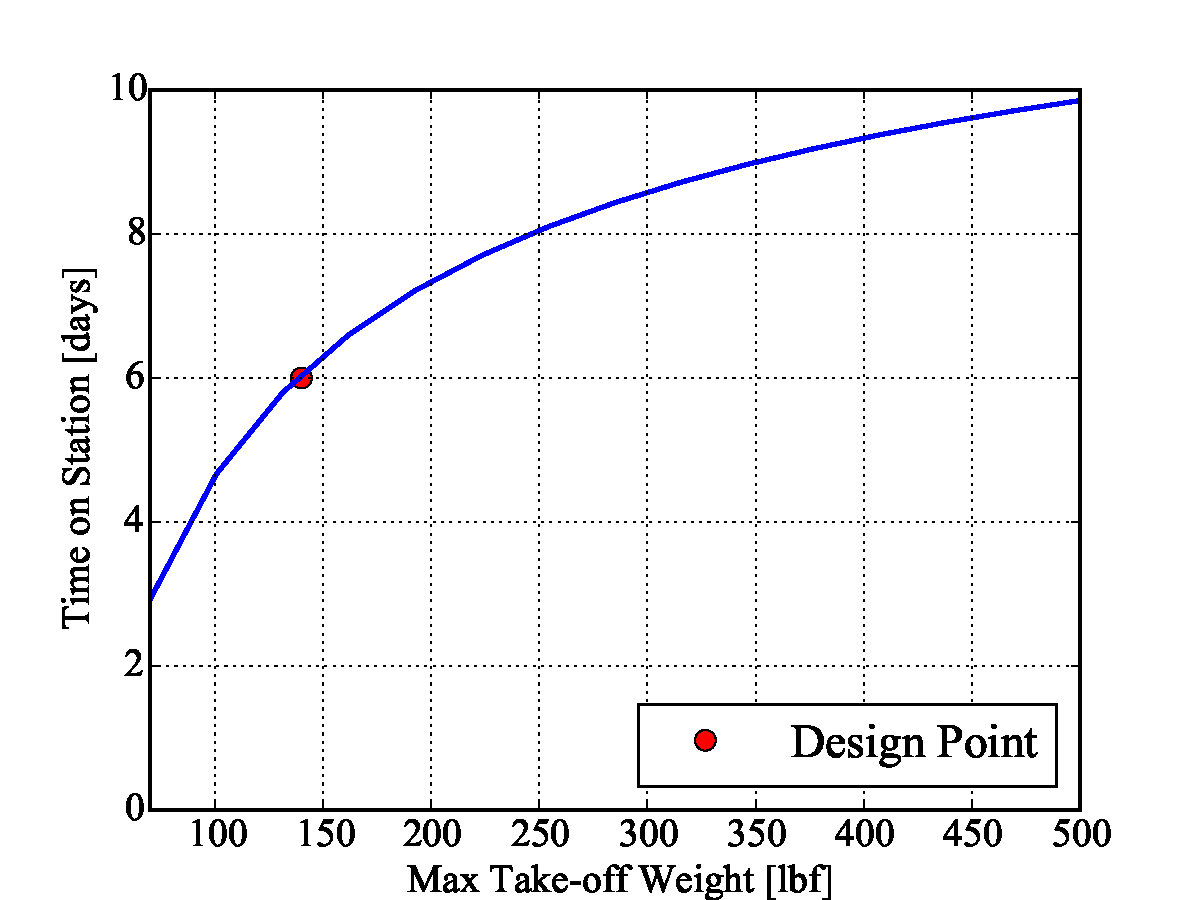
\includegraphics[width = .55\textwidth]{tvsmtow}
     \caption{ \textbf{Trade-off between MTOW and the time on station TO BE UPDATED} }
    \label{f:tvsmtow}
    \end{center}
\end{figure}

While more time on station could be achieved with larger aircraft, there are various downsides to larger aircraft in manufacturability, modularity, complexity, risk and cost. The design point of 5.6 days falls on the Pareto Frontier shown in Figure~\ref{f:tvsmtow}. 

Once the aircraft size was determined, the TP70 engine, a 70 cc single-cylinder four-stroke engine, was selected. It was determined to have the necessary power for the successful operation of the aircraft during all segments of the flight (discussed further in Section~\ref{a:propulsion}). Having chosen the engine, the aircraft was reoptimized with the fixed engine and constrained to fly for 5.65 days and the MTOW was minimized.  

\section{Aircraft Overview}
\label{Aircraft Overview}

The optimization discussed in Section~\ref{GPkit} results in the aircraft described in Figure~\ref{f:dimensions}. It is a 147 lb aircraft that is designed to fly for 5.65 days, and has a 63\% fuel fraction. 

\begin{figure}[H]
    \begin{center}
    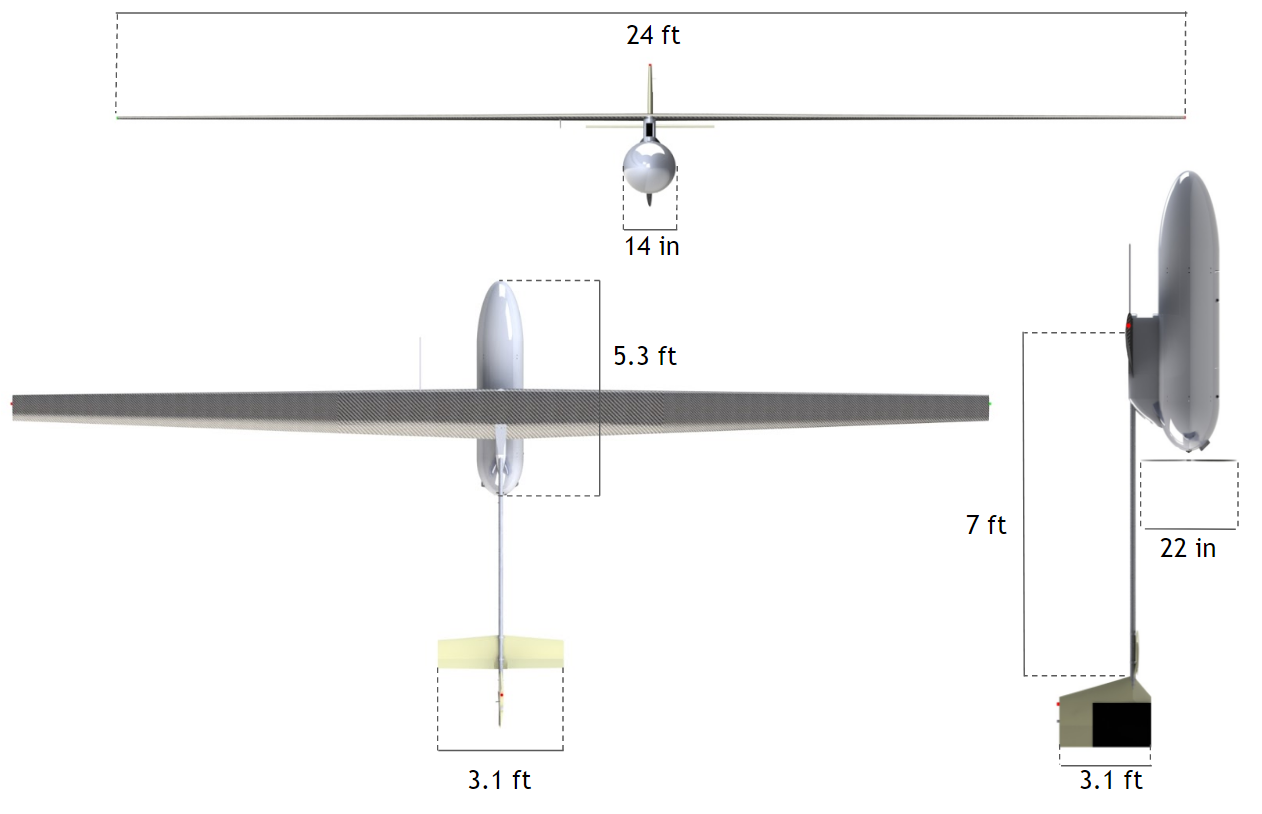
\includegraphics[width = .75\textwidth]{dimensions}
     \caption{ \textbf{Dimensional overview of the aircraft} }
    \label{f:dimensions}
    \end{center}
\end{figure}

The weight breakdown of the components within the aircraft is outlined in Figure \ref{f:weightBudget}. Since the first version of the aircraft is being prototyped at MIT, both the budgeted and actual weights of each component are listed. The prototype aircraft is 2 lbs lighter than the budgeted total weight of 147 lbs. 

\begin{figure}[H]
    \begin{center}
    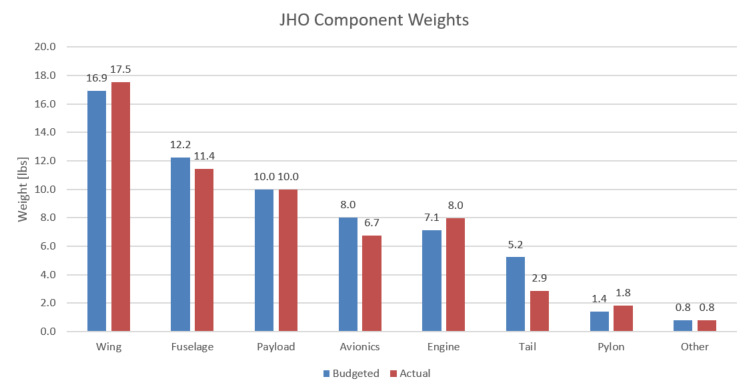
\includegraphics[width = .65\textwidth]{WeightBreakdown}
     \caption{ \textbf{Budgeted and actual weights of JHO subsystem components. Fuel has been omitted for graphical purposes, and weighs 86.3 lbs. The total weight of the components comes out at 145 lbs, 2 lbs lighter than the 147 lbs projected by the GP models.} }
    \label{f:weightBudget}
    \end{center}
\end{figure}

\subsection{V0, FAR107-Compliant Aircraft}

In an effort to be able to test the aircraft without having to do so at certified UAV test sites, the MIT 16.82 Flight Vehicle Engineering Team have devised a version of the JHO nicknamed the V0, that has a total weight of less than 55lbs. This aircraft, within Part 107 of the FAA Federal Aviation Regulations (FAR), can be operated at altitudes less than 400 feet above the ground, within line-of-sight of an appropriately-trained, land-based pilot. There are further restrictions of the aircraft operations to daylight hours with more than 3 miles of visibility. The purpose of the V0 will be to test flight-critical systems, including but not limited to controller tuning, autonomous operation, rate of fuel consumption, and engine and avionics cooling. 

The V0 achieves a takeoff weight of less than 55 lbs through the removal of the following components:
\begin{itemize}
	\item Alternator: Since the V0 will be operating for short durations (<1 hr), the systems can be run on the on-board battery. 
	\item Transponder and antenna: Satellite communications and the payload antenna are not required while in LOS flight. 
	\item Customer payload: The payload does not serve any useful functions at low altitude, and is deemed unnecessary for preliminary flight system tests. 
	\item Fuel tanks: The V0 will use a simple rigid fuel tank in the payload bay to save weight, and allow the aircraft to be statically stable with no payload. 
\end{itemize}

This configuration poses static margin challenges, since the removal of these components offsets the CG of the aircraft significantly aftward. It is likely that the configuration will require the addition of ballast on a boom extending out of the nose of the aircraft for better longitudinal stability. However, the V0 will allow for significant development and testing cost reductions, and is actively being built by the MIT 16.82 students. 

\section{Aircraft Performance}

This section details the endurance performance of the aircraft during off-design operations, predicted using the models created within the GPkit optimization framework. The off-design parameters considered are wind speed, payload weight, and payload power consumption. 

\subsection{Wind Speed vs. Endurance}
 Wind speed largely determines the availability because the aircraft has to be able to fly at least as fast as the wind speed in order to maintain coverage over the desired area. We compare how different wind speeds on station would affect the endurance of the aircraft. There are two flight patterns for the aircraft depending on the wind speed. Below a wind speed of 20 m/s, the aircraft will cruise at its maximum endurance speed of 20 m/s, and fly a standard racetrack holding pattern against the wind, as shown in Figure~\ref{f:tvsv_wind}, over its station. It means that the aircraft can loiter for up to 6.4 days in favorable (and nominal) wind conditions. Above 20 m/s, the aircraft will be flying directly into the wind and holding station in a hover, maintaining zero ground speed. The endurance of the aircraft drops below 5 days above 28 m/s winds.  

\begin{figure}[htbp!]
    \begin{center}
    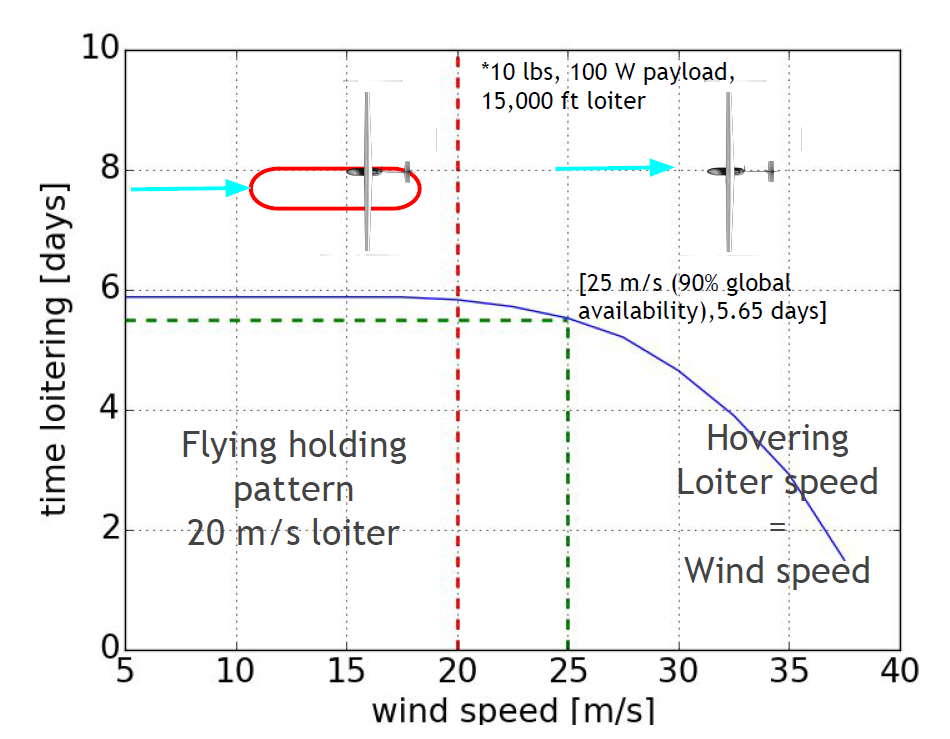
\includegraphics[width = .65\textwidth]{Vwind_vs_tstation}
     \caption{ \textbf{Performance curve of wind speed versus time on station.  For wind speeds below 20 m/s the plane will fly a holding pattern.  For wind speeds greater than 20 m/s the plane will fly directly into the wind, ``hovering" over its station .} }
    \label{f:tvsv_wind}
    \end{center}
\end{figure}

\subsection{Payload Weight vs. Endurance} 
Another performance study compares payload weight to endurance. The limiting factor on the payload weight of the aircraft is its longitudinal stability. The aircraft is designed to have a stability margin of 5\% with a 10 lb payload, which presents a good compromise between static stability and low trim drag during loiter. The aircraft is able to accommodate higher payloads with the same static margin by allowing for the addition of lead ballast in the tail boom, which offsets the forward CG shift due to changes in payload mass. This allows the longitudinal control characteristics of the aircraft to stay similar regardless of the payload size. 

 Figure~\ref{f:tvsw_pay} shows the relationship between endurance and payload weight, assuming loiter at 25 m/s at 15,000 ft. The red line shows the ballast required at different payload weights, which increases linearly. Due to the fact that the structure of the aircraft is designed , it is recommended that the payload weight of the JHO does not exceed 25 lbs. 

\begin{figure}[htbp!]
    \begin{center}
    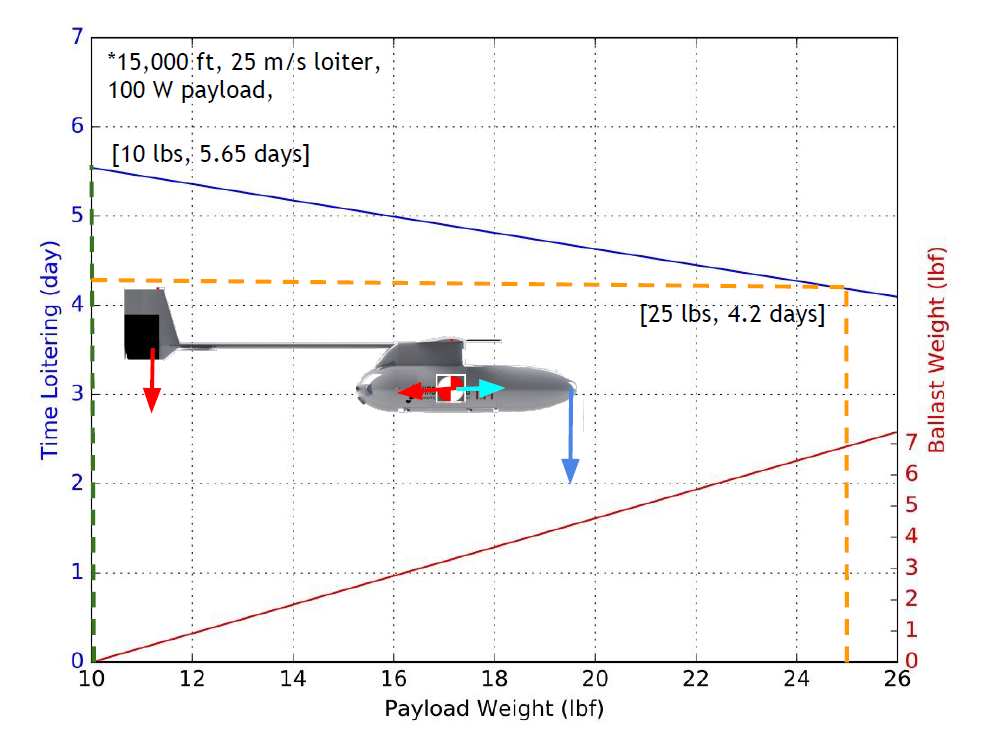
\includegraphics[width = .65\textwidth]{tvsw_pay}
     \caption{ \textbf{Performance curve of time on station versus payload weight.  The aircraft is designed to fly with a 10 lb payload, but can accommodate up to 25 lbs. This assumes that the payload volume is constant at 1.43 ft$^3$ regardless of payload weight. } }
    \label{f:tvsw_pay}
    \end{center}
\end{figure}

It is also important to note that, as payload weight varies, the structural margin of the aircraft also changes, and therefore would decrease at higher payloads. But since the aircraft was sized to a load factor of 5, this issue is minor.

\begin{figure}[!htbp]
    \begin{center}
    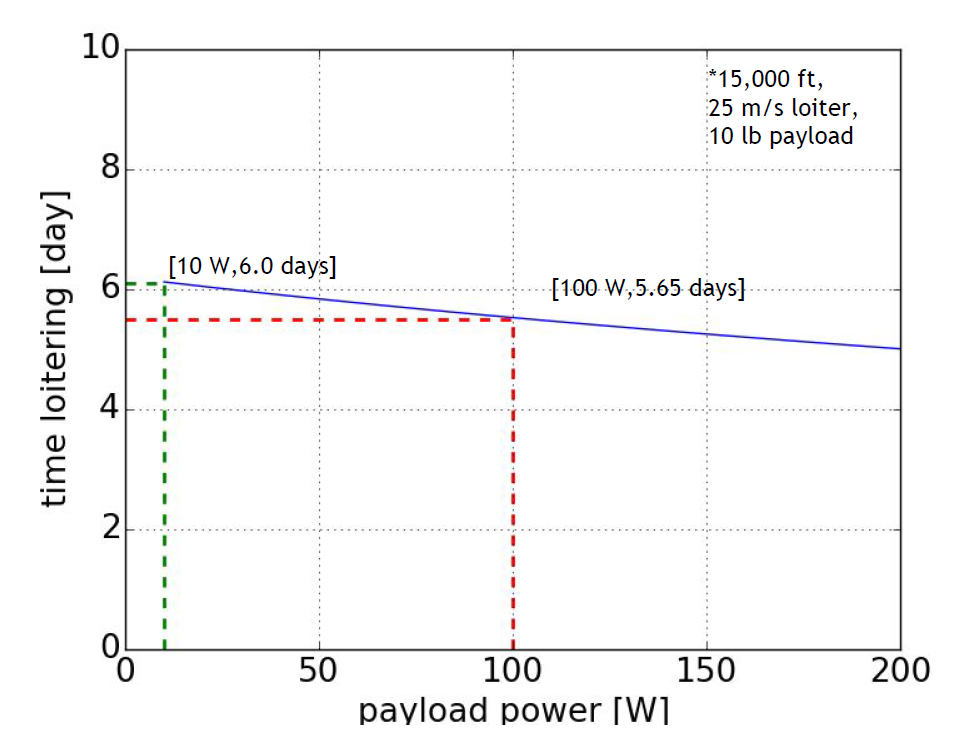
\includegraphics[width = .65\textwidth]{ppay_vs_tstation}
     \caption{ \textbf{Performance curve of time on station versus payload power. The aircraft achieves 6 days of endurance with a 10W payload, and 5.65 days with a 100W payload.} }
    \label{f:tvsP_pay}
    \end{center}
\end{figure}

\subsection{Payload Power vs. Endurance}

We examine the sensitivity of the aircraft endurance to the payload average power requirement, represented in Figure~\ref{f:tvsP_pay}. As shown, the aircraft can achieve 6 days of endurance with a 10W payload. While the aircraft can fulfill higher power requirements, the increased power draw results in a decrease in endurance. With a 100W payload, the aircraft can station-keep for 5.45 days. 

\section{Conclusion}

This paper proposes a novel aircraft concept designed to keep small payloads (~10lbs) aloft for 5.6 days in a cost-effective and robust package. Although this aircraft exists in a niche currently unoccupied by existing aircraft, the technologies present in it are low-risk and largely proven. While this aircraft has persistent communication coverage as its primary mission, its modularity enables it to accommodate a variety of payloads of varying size, weight, and power. The detailed design of this aircraft is underway at MIT, with a team of undergraduate and graduate students continuing work on the project as a part of the 16.82 Flight Systems Engineering Capstone subject. The project is being funded by the MIT Lincoln Labs and the Air Force, with the goal of having a flying prototype by the end of May 2017. The team is excited to have the opportunity to share preliminary test flight data for its V0 during the AIAA Aviation Conference. 

\section{Acknowledgements}

The authors would like to thank Professor Mark Drela, Professor John Hansman, Professor Warren Hoburg, and Jennifer Craig for their assistance and guidance with this project, as well as Hanscom Air Force Base and the MIT Lincoln Laboratory for their sponsorship and support. 

But most importantly, the authors would like to acknowledge their teammates in the 16.82 Flight Systems Engineering course at MIT who have worked, and are still striving to transform this aircraft from a concept into a working prototype. 

\section{Appendix}
\label{Appendix}

\subsection{Avionics}
\label{a:avionics}

Some of the key technologies that enable this kind of long endurance MALE UAV come from avionics. The avionics for the aircraft is a lightweight and low power package that has sufficient robustness and redundancy to complete many 5.65 day missions. The system is capable of attitude determination and control, autonomous mission control, UHF and SATCOM communication, and airspace integration.

A fully functional avionics package that weighs 6.7 lbs and draws a mean power of 40 W has been designed. The avionics hardware can be separated into functional groups (see Figure~\ref{f:blockdiag}) including sensors, control, central processing unit (CPU), communication, power management and extended items. These will be broken down below:

\begin{figure}[h!]
    \begin{center}
    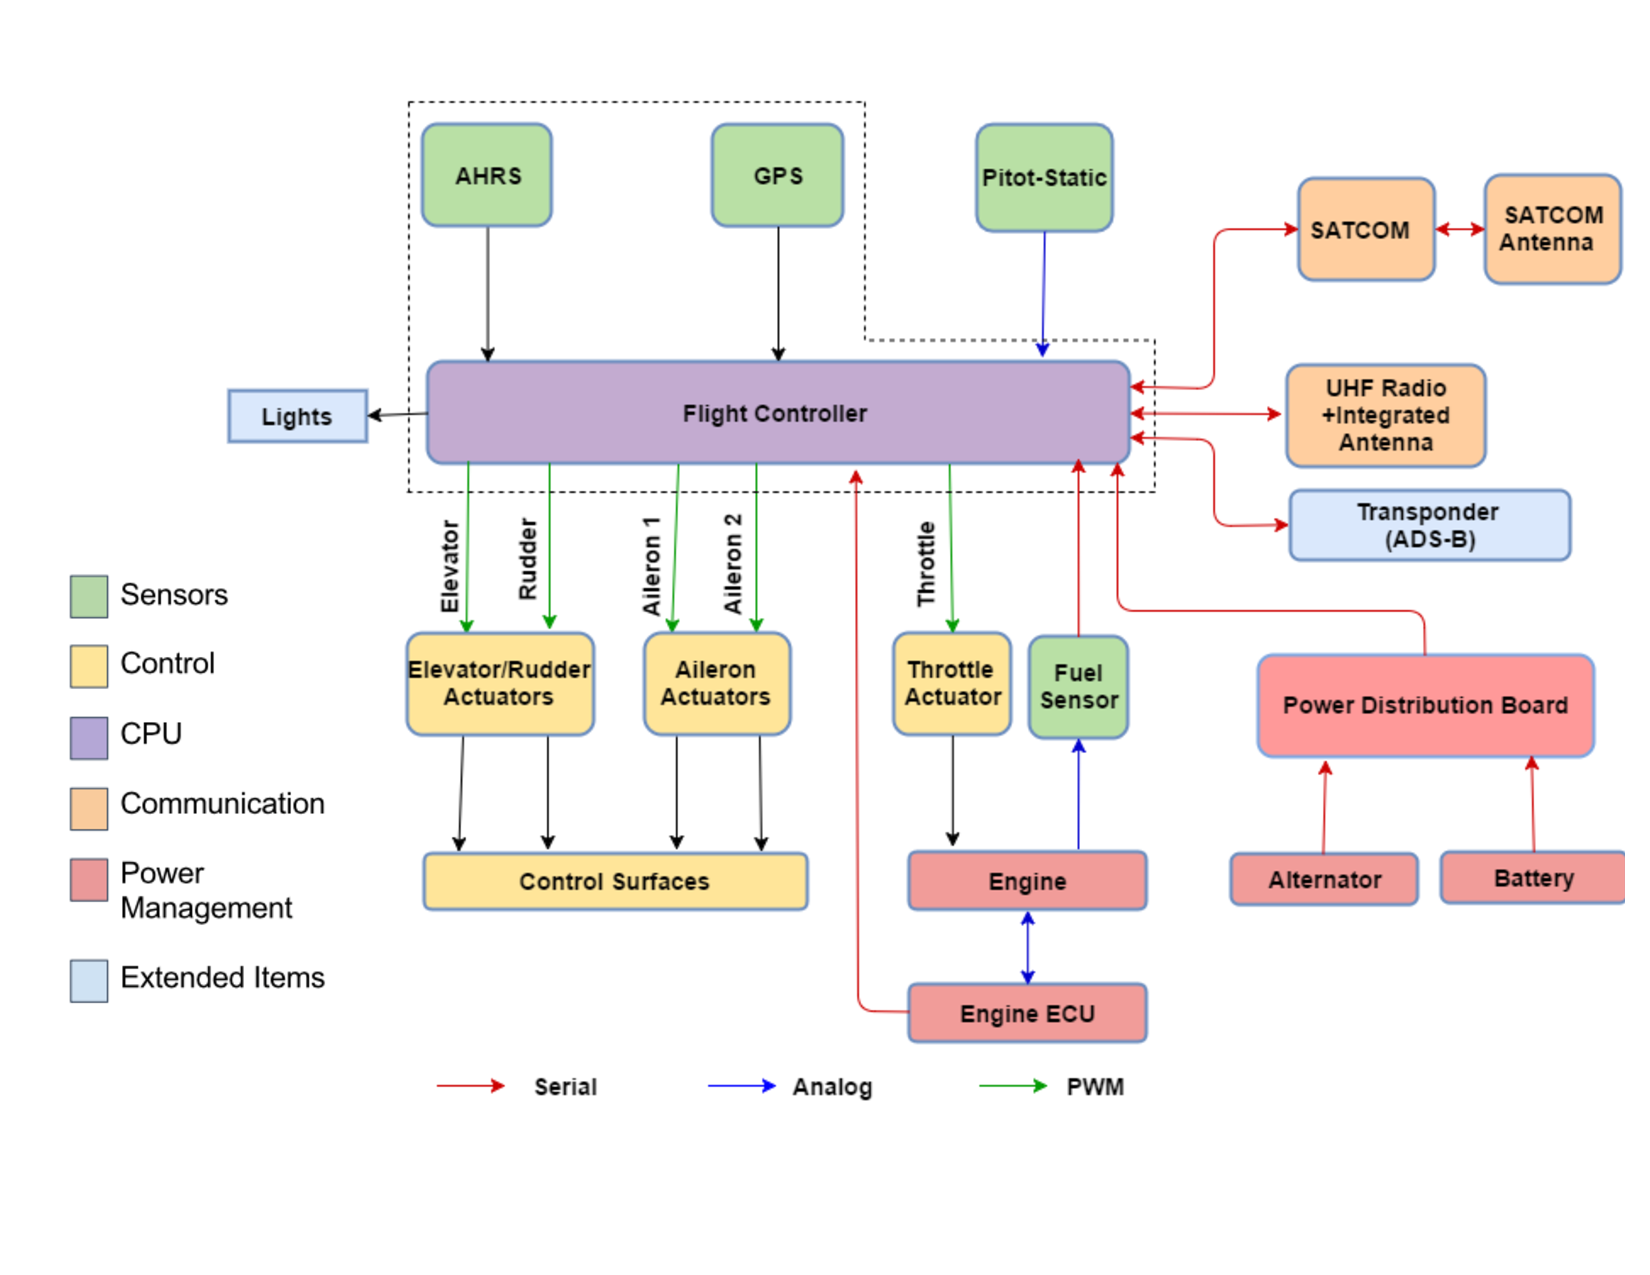
\includegraphics[width = .75\textwidth]{blockdiag}
     \caption{ \textbf{Avionics block diagram color-coded by functional area} }
    \label{f:blockdiag}
    \end{center}
\end{figure}

\begin{itemize}
    \item \textbf{Sensors: } The MicroPilot flight controller includes an on-board inertial navigation system. Other sensors include accelerometers, rate gyros, GPS, magnetometer, thermometer, and barometer. A pitot tube mounted on the wing provides the dynamic pressure, and two digital fuel sensors monitor fuel levels. 
    \item \textbf{On-board computing: } The MicroPilot flight controller is the primary computer for autonomous control, mission decisions including switching flight phases, failsafe modes, LOS control through the UHF link and BLOS communication. It also provides pulse width modulation (PWM) outputs for the eight-servo aircraft control system. 
    \item \textbf{Control: } Actuator sizing for a high endurance aircraft is a difficult task since servos tend to be the heaviest and most power hungry avionics components. The Pegasus actuators specified for this aircraft were sized to have exceptional reliability, and also support control surface deflections at never-exceed speed at MSL. 
    \item \textbf{Power distribution  management: } The power distribution and management system is responsible for supplying all required onboard power needs. It consists of an alternator, battery, and Power Management Unit (PMU). For power generation, a Sullivan UAV S676-300F-01~\cite{sullivan} alternator is specified. At loiter conditions (~4500 RPM), the alternator will be capable of delivering up to 220 W, satisfying all power requirements. An onboard 80 Wh lithium polymer battery provides fault-tolerance in the event of alternator or engine failure and ensures that high transient power loads do not cause momentary brown-outs. The battery's charge state is controlled by a battery management and power monitoring microcontroller, which submits diagnostic and monitoring information to the main flight computer.
    \item \textbf{Additional components} In order to comply with airspace integration requirements, the aircraft will include a Sagetech XPS-TR Mode S Transponder with Automatic Dependent Surveillance- Broadcast (ADS-B) Out. This transponder was chosen for its low size, weight, and power consumption as well as its capability of meeting the FAA's 2020 ADS-B requirements. Furthermore, there will be one light per wing (red on the port side and green on the starboard side) and a white strobe light on top.
    \item \textbf{Communication and ground station}
    The aircraft uses two modes of communication: a UHF two-way data radio for line-of-sight (LOS) and a satellite internet link (SATCOM) for beyond line-of-sight (BLOS). The ground station uses MicroPilot ground station control software, running on a laptop computer. Furthermore, for LOS control, a UHF radio controller is specified. Satellite communications capability is also required, and included in the ground station, to be able to contact Air Traffic Control in communications-denied areas. 
\end{itemize}

The physical configuration of the avionics bay is shown in Figure~\ref{f:avbay}.

\begin{figure}
	\begin{center}
		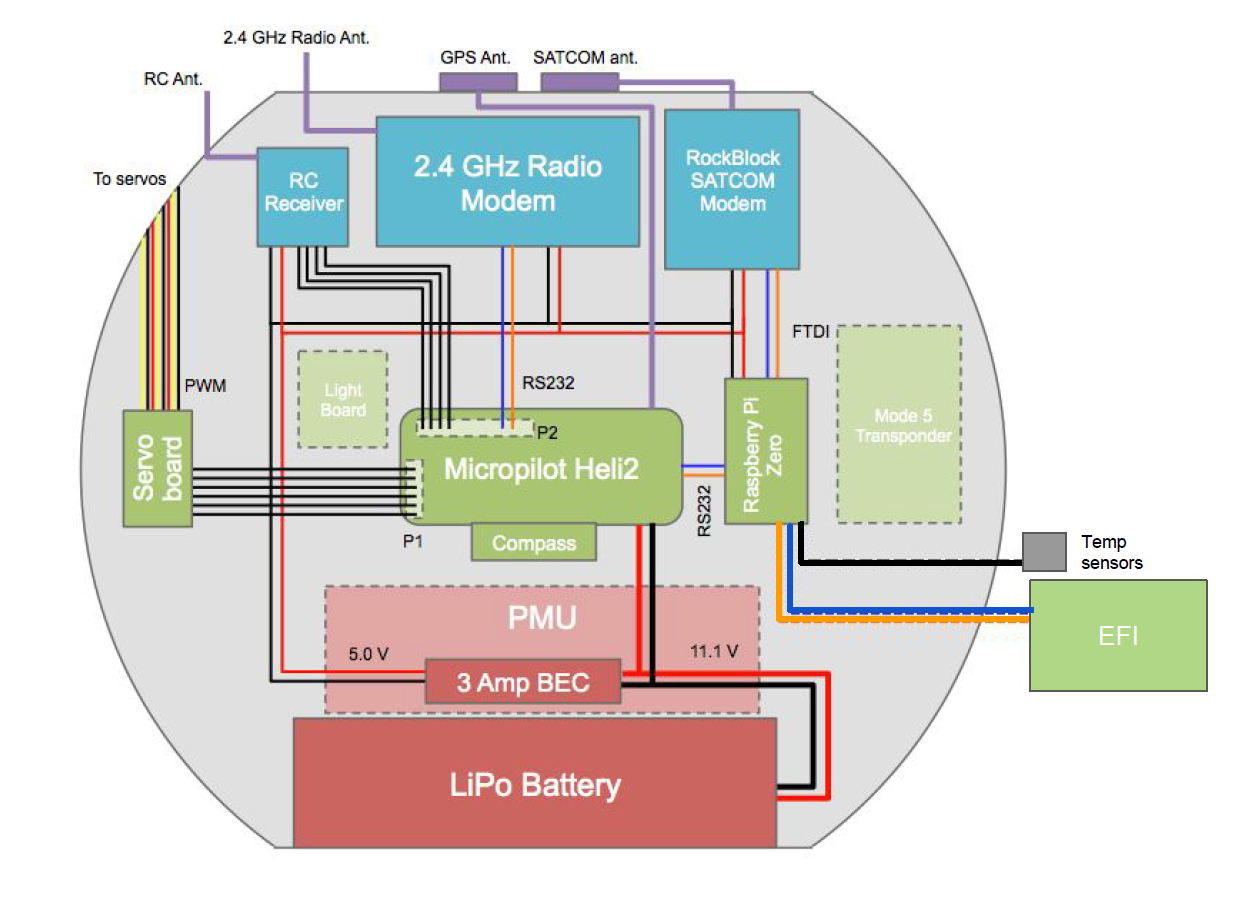
\includegraphics[width=.5\linewidth]{avbay.png}
		\caption{Physical layout of the avionics bay in front of the front bulkhead. Blue denotes communications, green control, red power system items.}
		\label{f:avbay}
	\end{center}
\end{figure}

\subsection{Propulsion}
\label{a:propulsion}

There were two proposed engine options for the JHO, which were the RCV Engines DF70, a two piston, four stroke engine, and the TorqPro TP70, a single piston, four stroke engine. Each of these engines meet both the propulsive and electric power requirements of the aircraft. The TP70 engine was chosen due to its significantly lower cost and shorter lead time compared to its two-piston counterpart. The engine was ordered, and fitted with a COTS electronic fuel injection (EFI) system. Preliminary BSFC tests for the TP70 demonstrate similar performance characteristics for this engine vs. its counterpart, validating the engine choice. 

\begin{figure}
	\centering
	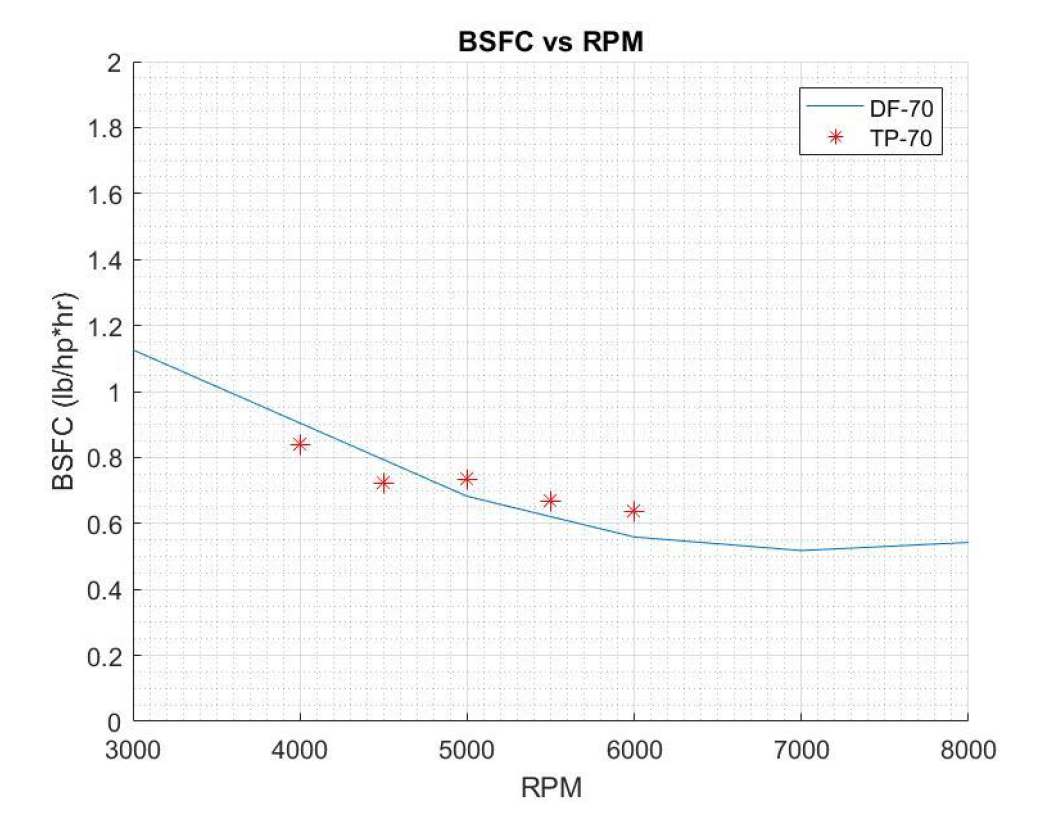
\includegraphics[width=.5\linewidth]{BSFCvalidation.png}
	\caption{BSFC ground test data for the TP70, overlaid on the manufacturer-provided performance data for the DF70.}
	\label{f:BSFCvalidation}
\end{figure}

The engine runs on 100ll aviation gasoline, with a 50:1 fuel/oil ratio.  The fuel circuit is a conventional electronic fuel injection circuit, with a high pressure fuel pump drawing fuel from two main fuel tanks. A 22"x8" propeller was chosen by considering both takeoff, top-of-climb, and loiter thrust requirements. It was confirmed that the engine and propeller combination could meet the BSFC and thrust requirements at every phase of the mission. 
    
\subsection{Modularity}
\label{a:modularity}

With modularity in mind, the aircraft was designed to disassemble along breakpoints, and fit within a 108"x24"x22" box for storage and transportation. This scheme is shown in Figure~\ref{f:modularity}.

\begin{figure}[h!]
\centering
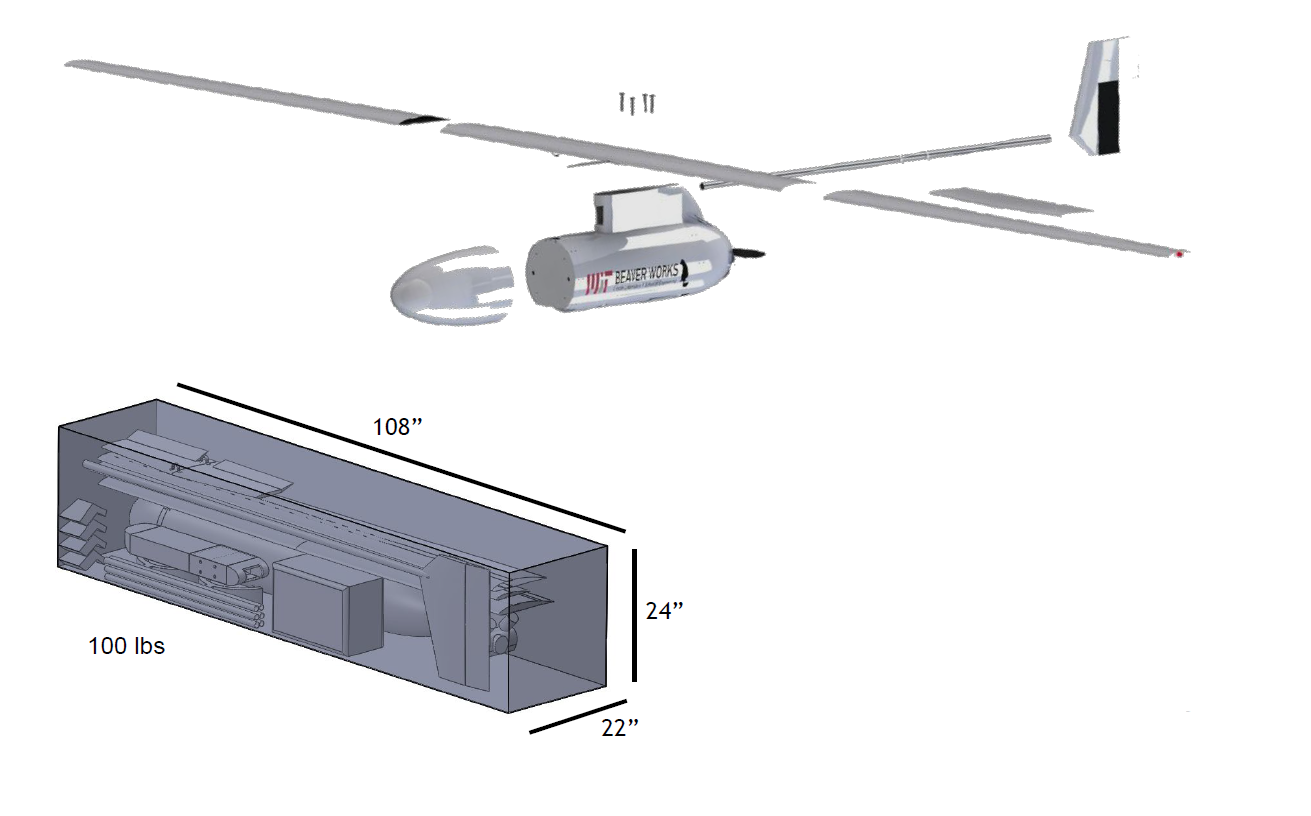
\includegraphics[width=.5\linewidth]{modularity.png}
\caption{Aircraft breakpoints and packing configuration}
\label{f:modularity}
\end{figure}
    

\bibliographystyle{aiaa}
\bibliography{biblibrary}

\end{document}